% Options for packages loaded elsewhere
\PassOptionsToPackage{unicode}{hyperref}
\PassOptionsToPackage{hyphens}{url}
\PassOptionsToPackage{dvipsnames,svgnames,x11names}{xcolor}
%
\documentclass[
  12pt,
]{article}
\usepackage{amsmath,amssymb}
\usepackage{iftex}
\ifPDFTeX
  \usepackage[T1]{fontenc}
  \usepackage[utf8]{inputenc}
  \usepackage{textcomp} % provide euro and other symbols
\else % if luatex or xetex
  \usepackage{unicode-math} % this also loads fontspec
  \defaultfontfeatures{Scale=MatchLowercase}
  \defaultfontfeatures[\rmfamily]{Ligatures=TeX,Scale=1}
\fi
\usepackage{lmodern}
\ifPDFTeX\else
  % xetex/luatex font selection
\fi
% Use upquote if available, for straight quotes in verbatim environments
\IfFileExists{upquote.sty}{\usepackage{upquote}}{}
\IfFileExists{microtype.sty}{% use microtype if available
  \usepackage[]{microtype}
  \UseMicrotypeSet[protrusion]{basicmath} % disable protrusion for tt fonts
}{}
\makeatletter
\@ifundefined{KOMAClassName}{% if non-KOMA class
  \IfFileExists{parskip.sty}{%
    \usepackage{parskip}
  }{% else
    \setlength{\parindent}{0pt}
    \setlength{\parskip}{6pt plus 2pt minus 1pt}}
}{% if KOMA class
  \KOMAoptions{parskip=half}}
\makeatother
\usepackage{xcolor}
\usepackage[left=1in,right=1in,top=1in,bottom=1in]{geometry}
\usepackage{graphicx}
\makeatletter
\def\maxwidth{\ifdim\Gin@nat@width>\linewidth\linewidth\else\Gin@nat@width\fi}
\def\maxheight{\ifdim\Gin@nat@height>\textheight\textheight\else\Gin@nat@height\fi}
\makeatother
% Scale images if necessary, so that they will not overflow the page
% margins by default, and it is still possible to overwrite the defaults
% using explicit options in \includegraphics[width, height, ...]{}
\setkeys{Gin}{width=\maxwidth,height=\maxheight,keepaspectratio}
% Set default figure placement to htbp
\makeatletter
\def\fps@figure{htbp}
\makeatother
\setlength{\emergencystretch}{3em} % prevent overfull lines
\providecommand{\tightlist}{%
  \setlength{\itemsep}{0pt}\setlength{\parskip}{0pt}}
\setcounter{secnumdepth}{5}
\usepackage{sectsty}
\usepackage{setspace}\spacing{1}
\usepackage{float}
\usepackage{fancyhdr}
\usepackage{mathtools}
\usepackage{algorithm,algpseudocode,caption}
\usepackage{natbib}\bibliographystyle{apalike}
\usepackage[nottoc, numbib]{tocbibind}
\usepackage{paralist}
\usepackage{verbatim}
\usepackage{comment}
\usepackage{soul}
\usepackage{array}
\ifLuaTeX
  \usepackage{selnolig}  % disable illegal ligatures
\fi
\IfFileExists{bookmark.sty}{\usepackage{bookmark}}{\usepackage{hyperref}}
\IfFileExists{xurl.sty}{\usepackage{xurl}}{} % add URL line breaks if available
\urlstyle{same}
\hypersetup{
  colorlinks=true,
  linkcolor={Maroon},
  filecolor={Maroon},
  citecolor={Blue},
  urlcolor={blue},
  pdfcreator={LaTeX via pandoc}}

\author{}
\date{\vspace{-2.5em}}

\begin{document}

\pagenumbering{gobble}
\allsectionsfont{\normalsize\bfseries}
%%%%%%%%%%%%%%%%%%%%%%%%%%%%%%%%%%%%%%%%%%%%%%%%%%%%%%%%%%%%%%%%%%%%%%%%%%%%%%%%%%%%%%%%%%%%%%%%%%%%%%%%%%%%%%%%

%\begin{titlepage}
\begin{center}
\vspace*{.5in} %this seems to work to get the 2in margin on title page
\doublespacing
\Large{\textsc{Capture-Recapture with Covariates: The Bayesian Logistic Capture-Recapture Model with Extensions}}\\
\vspace*{5\baselineskip}
\normalsize{Robert Edward Granger}\\
\vspace*{7.5\baselineskip}
\singlespacing
\normalsize{Submitted to the faculty of the Univesity Graduate School \\
in partial fulfillment of the requirements \\
for the degree \\
Doctor of Philosophy \\
in the Department of Statistics, \\
Indiana University \\
May 2024 (set this to month in which all requirements are fulfilled in title.sty)}
\end{center}
% \end{titlepage}

\hypersetup{linkcolor = black}
\pagenumbering{roman}
\thispagestyle{empty}
\newpage

%%%%%%%%%%%%%%%%%%%%%%%%%%%%%%%%%%%%%%%%%%%%%%%%%%%%%%%%%%%%%%%%%%%%%%%%%%%%%%%%%%%%%%%%%%%%%%%%%%%%%%%%%%%%%%%%%%%
%%%%%%%%%%%%%%%%%%%%%%%%%%%%%%%%%%%%%%%%%%%%%%%%%%%%%%%%%%%%%%%%%%%%%%%%%%%%%%%%%%%%%%%%%%%%%%%%%%%%%%%%%%%%%%%%%%%%
\singlespacing

Accepted by the Graduate Faculty, Indiana University, in partial fulfillment of the requirements for the degree of Doctor of Philosophy.

\vspace*{6\baselineskip}

\begin{tabular}
{>{\raggedright\arraybackslash}p{1.5in}
 >{\raggedleft\arraybackslash}p{4.75in}}
Doctoral Committee: & \hrulefill \\
& Daniel Manrique-Vallier, Ph.D. \\
\\
\\
& \hrulefill \\
& Julia Fukuyama, Ph.D. \\
\\
\\
& \hrulefill \\
& Amanda Mejia, Ph.D. \\
\\
\\
& \hrulefill \\
& Roni Khardon, Ph.D. \\
\end{tabular}

\vspace*{20\baselineskip}

\raggedright

May 1, 2024 (change this to defense date, it's in title.sty)

\newpage
%%%%%%%%%%%%%%%%%%%%%%%%%%%%%%%%%%%%%%%%%%%%%%%%%%%%%%%%%%%%%%%%%%%%%%%%%%%%%%%%%%%%%%%%%%%%%%%%%%%%%%%%%%%%%%%%%%%%
\doublespacing
\begin{center}
Robert Edward Granger\\
\textsc{Capture-Recapture with Covariates: The Bayesian Logistic Capture-Recapture Model with Extensions}\\
\end{center}

\normalsize

Capture-recapture refers to a series of methods that are used to estimate the size of a population from at least two incomplete, matched lists.  With human populations, heterogeneity in the capture probability is a serious concern as it can impact the estimation process. This proposal outlines a framework for incorporating heterogeneity through known covariates into the estimation process and develops an extensible model under this framework which we call the Bayesian Logistic Regression model for Capture-Recapture (BLRCR). The posterior distribution is estimated using the complete likelihood through a Markov Chain Monte Carlo (MCMC) algorithm.  Through a careful examination of the problem and a series of demonstrations, three important areas of future research become apparent for the dissertation project. First, we should consider the impact of the specification of the covariate distribution and explore additional non-parametric solutions.  Second, we should consider the unobserved heterogeneity and specifically how to implement a procedure that accounts for this violation in the conditional independence assumption.  Third, we should consider the impact of variable selection.

\newpage
%%%%%%%%%%%%%%%%%%%%%%%%%%%%%%%%%%%%%%%%%%%%%%%%%%%%%%%%%%%%%%%%%%%%%%%%%%%%%%%%%%%%%%%%%%%%%%%%%%%%%%%%%%%%%%%%%%%%
\tableofcontents
\newpage
%%%%%%%%%%%%%%%%%%%%%%%%%%%%%%%%%%%%%%%%%%%%%%%%%%%%%%%%%%%%%%%%%%%%%%%%%%%%%%%%%%%%%%%%%%%%%%%%%%%%%%%%%%%%%%%%%%%%

\pagenumbering{arabic}
\hypersetup{linkcolor = blue}

\pagenumbering{arabic}

\newpage
\section{Introduction}
\label{sec:Introduction}

Capture-Recapture (CR) refers to a series of methods that are used to
estimate the size of a population from at least two incomplete, matched
lists. While one could simply count the number of unique names between
the lists, this would provide only a lower bound estimate of the
population size. Presumably, there are individuals who were not captured
in any of the lists. CR methods use assumptions along with patterns in
the data to create estimates for how many individuals were missed and
therefore inherently the size of the total population.

Most early applications of capture-recapture, also called mark and
recapture, were in the context of animal populations where a number of
animals were initially captured, marked or tagged, and then released.
This was followed up with another capturing occasion where animals were
captured and checked for a marking. A CR dataset is then a listing of
each unique animal's capture pattern after all sampling occasions have
taken place. CR methods have been used in a wide array of additional
subject areas including ecology \citep{henderson_ecological_2016},
epidemiology \citep{goldberg_estimation_1978,baker_simple_1990}, U.S.
Census adjustments \citep{darroch_three-sample_1993}, and estimating the
number of pages on the internet
\citep{lawrence_searching_1998,khabsa_number_2014}. Of particular
interest to this dissertation is the application of this methodology to
human populations, which are sometimes referred to as multiple systems
estimation (MSE). Lists of subjects may be collected by various
institutions including hospitals, government agencies, or other
non-governmental organizations but are left incomplete due to lack of
resources, mistakes/omissions, or just the inability to obtain such
information. These lists can then be combined and constructed to form a
dataset for CR. For example, \cite{zwane_population_2005} attempts to
determine the number of Dutch children born with a neural tube defect
(NTD) in the year 2000 by analyzing three national databases tracking
these occurrences. For multiple reasons including risk assessment of the
pregnancy and omissions, not all children with NTDs are reported to each
database. Another example is the counting of casualties from various
conflicts including Colombia
\citep{guberek_count_2010,manriquevallier_bayesian_2016}, Guatemala
\citep{ball_making_2000,ball_statistics_2018}, Kosovo
\citep{ball_killings_2002,manriquevallier_bayesian_2016}, Peru
\citep{ball_estimate_2003}, and many others. Casualty counts by a
reporting agency may only be partially collected because of
non-cooperation from victims due to lack of trust, danger posed to data
collectors, and/or destroyed infrastructure
\citep{manrique-vallier_capture-recapture_2020}.

CR methods often come with many assumptions including a closed
population, independence between lists, and homogeneity in the capture
probability between individuals. In particular, the aim of the
dissertation is to extend methods that target the homogeneity
assumption, the requirement that all individuals have the same
probability of capture on each list regardless of any personal
attributes. While this may be a palatable assumption for some animal
populations, this is unlikely with human populations. Different
characteristics like age or social status may influence the probability
of their capture. If data is present that can fully explain the
heterogeneity, one could incorporate this by stratifying before applying
their CR method of choice
\citep{sekar_method_1949,manrique-vallier_estimating_2019}. This is only
possible if the covariate is discrete or can be made discrete. It can
also lead to issues of sparsity. An alternative is to include the
covariates in a model like regression
\citep{alho_logistic_1990,baker_simple_1990,bonner_mcmcmc_2014,king_capturerecapture_2016}.
Regardless, this only addresses the observable heterogeneity and ignores
heterogeneity that may exist but covariate information is missing or is
not fully adequate. Some approaches have been proposed to account for
unobservable heterogeneity by adapting the Rasch model
\citep{darroch_three-sample_1993} or latent class memberships
\citep{manriquevallier_bayesian_2016}.

This dissertation develops a fully Bayesian procedure for the CR problem
that has a number of desirable characteristics:

\begin{itemize}

\item[1)] allows for multiple lists;
\item[2)] is resistant to sparsity;
\item[3)] can be informed through the use of priors;
\item[4)] uses discrete and continuous covariates to account for observable heterogeneity;
\item[5)] can also account for unobservable heterogeneity;
\item[6)] extensible;

\end{itemize}

Estimating the size of the population tends to be highly susceptible to
the structure of the modeling when dealing with CR methods. Therefore,
implementing covariates in an improper way or not adequately accounting
for the unobservable heterogeneity can bias the inference. As a result,
we propose developing a method that is fully Bayesian approach and uses
the full likelihood as suggested by \cite{pollock_use_2002}. We begin by
developing a framework for CR that incorporates covariates, a framework
that for all intents and purposes is identical to the complete
likelihood specification in \citep{king_capturerecapture_2016}. Using
this framework, we specify a model that uses conditionally independent
logistic regressions which we term the Bayesian Logistic Regression
Capture-Recapture (BLRCR) model.

While the BLRCR model incorporates individual covariates and thus
accounts for observable heterogeneity, it has a few shortcomings:

\begin{list}{}{}
\item[1)] Since covariates are missing at least for the unobserved individuals, the use of a full likelihood approach requires the specification of a distribution for the covariates. As we will see in Section \ref{Sec:selectcovariates}, misspecifying the distribution can lead to incorrect inference. Like previous approaches, we apply a normal distribution; however, we propose a new method of using non-parametric approaches to the covariates such as an infinite mixture of normal distributions.

\item[2)] Unobservable heterogeneity can bias the inference, and hence we need a way to account for it. From our perspective, we view the idea of unobservable heterogeneity as an issue of omitted covariates. We borrow the idea of individuals belonging to latent classes impacts the probability of capture\citep{manriquevallier_bayesian_2016}, but implement it in the regression procedure through an additional intercept term. 

\item[3)] Determining which covariates to include and how each covariate should be included in the regression will ultimately impact the inference. There are multiple ways to account for this issue, but we explore it through the lens of variable selection. We investigate the difficulty of computing the Bayes Factor and ultimately suggest a regularization technique.

\end{list}

The dissertation proceeds as follows: Section \ref{Sec:litreview}
provides a brief history of the capture-recapture problem while
reviewing literature relevant to Bayesian and covariate extensions.
Section \ref{sec:CRwithCovariates} begins with preliminary details,
provides a model using conditional independent Bayesian Logistic
Regressions, and approximates the posterior distribution using a Markov
Chain Monte Carlo (MCMC) estimation procedure. Section
\ref{Sec:selectcovariates} explores different covariate distributions
along with nonparametric specifications. Section
\ref{Sec:condindependence} introduces hidden covariates that allow for a
breaking of the conditional independence assumption. Section
\ref{Sec:modelselection} investigates the problem of model selection.
Section \ref{Sec:example1} looks at Example 1. Section
\ref{Sec:example2} looks at Example 2. Section \ref{Sec:Conclusion}
concludes with a summary of the dissertation and future directions of
work in this area.

\newpage
\section{Literature Review}
\label{Sec:litreview}

Capture-Recapture (CR) refers to a series of methods that are used to
estimate the size of a population from at least two incomplete, matched
lists. This naming comes from the process of first capturing/marking a
number of organisms (capture) and following up with a second capturing
occasion (recapture). One then estimates the population size, \(N\), of
the organism by comparing the number of organisms marked in each sample,
\(n_1\) and \(n_2\), and the organisms that were matched in both
samples, \(n_{12}\). Intuitively, the proportion of the total population
that is initially captured/marked, \(n_1/N\), should be equal to the
proportion of captured/marked individuals that are recaptured,
\(n_{12}/n_2\). Of course, this only makes sense if we believe the lists
are independent. Rearranging and solving for \(N\) leads to the formula:

\[\hat{N} = \frac{n_1 \cdot n_2}{n_{12}}.  \]

Although this estimator was used as early as 1783 by the mathematician
Pierre-Simon Laplace for the purpose of estimating the French population
\citep{schaefer_estimation_1951}, this estimator is commonly referred to
as the Lincoln-Petersen estimator after its early use by Frederick C.
Lincoln on migratory waterfowl \citep{lincoln_calculating_1930} and C.G.
Johannes Petersen on the fish species plaice
\citep{petersen_yearly_1895}. The Lincoln-Petersen estimator is
relatively simple to compute, but is limited to only two lists with the
assumption of a closed population. A closed population means the
population does not change throughout the sampling occasions. This
estimator also makes two other intricately related assumptions:

\begin{list}{}{}

\item[1)] independence between lists,

\item[2)] homogeneity in capture probabilities between individuals.

\end{list}

The first assumption of independence between lists means the probability
an individual is captured on one list does not dependent on the
probability that individual is captured on another list. The second
assumption means the probability of any two individuals being captured
on a list is the same. When these assumptions are violated, it can lead
to bias in our population estimates. Addressing violations of these
assumptions has a long history and continues to be looked into today.

\subsection{Early Approaches to List Dependency and Homogeneity}
\label{sec:earlyapproachlitreview}

Capture-recapture solutions with multiple lists appear at least as early
as the 1920s
\citep{geiger_zahl_1924,schnabel_estimation_1938,darroch_multiple-recapture_1958}.
All use a model for estimating the size of a population from multiple
lists with list independence. If this assumption were to hold, then the
probability an individual appears on one list would not impact the
probability that the individual appears on another list. Perhaps for
carefully controlled experiments, list independence can be assumed, but
for most real applications, this is unlikely. For example with human
rights data, this may be violated as psychological research indicates
survivors of human rights abuses can benefit in their mental health by
sharing their testimony. These individuals may in turn be encouraged to
share their experiences to multiple outlets. Furthermore, there is
evidence with the Guatemalan Civil War that several popular movements
groups encouraged their social bases to provide testimony of human
rights abuses to all of three of the data collecting organizations
\citep{ball_making_2000}. These conditions lead to positive list
dependence and therefore an underestimate of the population size. On the
other hand, there is also the potential that certain groups of
individuals may feel uneasy sharing their testimony with non-aligned
data collection groups, leading to negative dependence and an
overestimate of the population size. For example, religious members of
the Catholic faith were more apt to give their testimony to the Catholic
researchers than they were to the political left, non-governmental
organizations \citep{manrique-vallier_capture-recapture_2020}.

In the early 1970s, two approaches were developed to address list
dependency. \cite{fienberg_multiple_1972} addressed the issue of list
dependency directly by modeling interactions between lists using
hierarchical log linear models under a multinomial sampling scheme. On
the other hand, \cite{sanathanan_models_1972} also used a multinomial
sampling scheme but instead of modeling list dependence directly, she
modeled it as unobserved heterogeneity in the individuals under a
conditional likelihood approach. As pointed out in several places
\citep{darroch_three-sample_1993,fienberg_classical_1999,manrique-vallier_capture-recapture_2020},
list dependency and heterogeneity between individuals are intricately
related such that list dependency can be viewed as a result of
heterogeneity between individuals. This leads to the second assumption,
homogeneity, which refers to all individuals having the same capture
probability within a list. For a variety of reasons, we may expect
certain individuals to be more likely to be captured because of
characteristics like geographic area, age, or their status within the
community.

This heterogeneity among individuals may be unobserved, observed through
covariates, or a combination. In the 1990s, various methods were
proposed to account for unobserved heterogeneity using adaptations to
log-linear and mixture models
\citep{darroch_three-sample_1993,agresti_simple_1994,pledger_unified_2000}.
Later, Bayesian methods based on latent class models were presented that
allowed for a more flexible approach to heterogeneity
\citep{fienberg_classical_1999,manrique-vallier_population_2008,manriquevallier_bayesian_2016}.
These methods seek out patterns in the capture histories in order to
infer for unobserved heterogeneity. When the researcher has accompanying
discrete covariate data, a suggestion noted by
\cite{darroch_three-sample_1993}, is to first stratify the data based on
the observable heterogeneity \citep{sekar_method_1949}, and then perform
the desired method within that stratification. An example of this this
implementation can be found in \cite{manrique-vallier_estimating_2019},
where the authors estimate the number of casualties in the internal
conflict in Peru (1980-2000) based on geographic stratifications.
Stratification becomes problematic in the presence of continuous
covariates. When continuous covariates are present, the researcher must
make difficult decisions on how to discretize the covariates which leads
to assigning potentially arbitrary cutoffs. If your stratification
scheme results in too many strata, the number of observed individuals
within each strata may be small, resulting in loss of inferential power
and identifiability. These issues can arise even without continuous
covariates if there are many discrete variables with many unique levels.

\subsection{Capture-Recapture with Covariates}

An alternative to stratification is to use the covariates within the
modeling process like with regression. \cite{pollock_use_1984} suggested
the use of logistic regression with environmental and individual level
covariates. \cite{huggins_statistical_1989,alho_logistic_1990}
independently proposed a similar but slightly different approach that
uses conditional maximum likelihood logistic regression through a two
step process. First, the coefficients for the logistic regression model
are obtained by regressing whether the individual was captured against
the covariates under the condition the individual is observed at least
once. If we perform the regression without taking into account that only
observed individuals appear in the dataset, i.e., some individuals are
missing, the coefficients become biased. After obtaining the
coefficients, we fit the probability that each individual is captured on
each list, and the probability an individual is missing, \(\theta_i\),
is computed. The second step uses the estimated probability of missing
by plugging it into the \cite{horvitz_generalization_1952} estimator,

\begin{equation*}
\hat{N} = \sum_i^n \frac{1}{\theta_i},
\end{equation*}

to obtain an estimate for \(N\). Intuitively, the estimator inverts the
probability of missing to account for the number of similar individuals
that would have been unobserved. This intutition implies that the
estimator will not perform well when the covariates for the observed
individuals vary significantly from the unobserved individuals.
Nevertheless, \cite{alho_logistic_1990} shows this estimator to be
consistent with large samples and develops an asymptotic approach to
estimating the variance.

In these models, the probability an individual is captured on each list
is conditionally independent of the other lists conditional on the
covariates. While covariates may explain some of the heterogeneity, it
is unlikely that all heterogeneity between individuals can be explained
in such a fashion and that some list dependency would not remain.
\cite{zwane_population_2005} use multinomial logistic regression with a
design matrix intended to directly model the dependence between the
lists. One could theoretically incorporate additional rows into the
design matrix to account for unobserved heterogeneity as in
\cite{darroch_three-sample_1993}.

Since the covariates will be missing for any of the unobserved
individuals, any approach that uses the complete likelihood would
require the covariate distribution to be specified. All of the previous
mentioned methods sidestep this need by maximizing the conditional
likelihood instead of the full likelihood.
\cite{stoklosa_heterogeneous_2011} takes this a step further by
comparing a partial likelihood approach, i.e, the number of recaptures
after the first capture, with the conditional approach. They find a loss
of efficiency but argue that it allows more flexibility in modeling.
Later, \cite{yee_vgam_2015} presented a simple way to implement
conditional likelihood methods using the \texttt{VGAM} package in the
programming software \texttt{R}. There is some early usage of a full
likelihood approach appearing in work that combines line transact theory
with capture-recapture for population estimation
\citep{alpizar-jara_combination_1996,borchers_mark-recapture_1998}.
Since the full likelihood approach requires specifying a distribution
for the covariates, this presents the difficulty of potentially
estimating additional parameters regarding the covariate distribution
and/or integrating out the covariates to obtain an estimate for \(N\).
While more challenging, \cite{pollock_use_2002} speculates the full
likelihood approach could result in better precision and suggests a
possible solution may lie with Bayesian methods.

\subsection{Bayesian Methods for Capture-Recapture}

Perhaps the earliest paper to utilize Bayesian methods is
\cite{roberts_informative_1967} in the evaluation of ``stopping rules''
with exactly two samples. The ``stopping rule'' refers to how the sample
of individuals from the population will be collected, and in particular,
what criterion must be met before concluding the sampling occasion. For
example, a researcher may choose a fixed sample size and will stop
sampling subjects when this sample size is reached. On the other hand,
the researcher may attempt to sample every subject within a fixed time
period. Depending on the chosen stopping rule, the likelihoods can
differ and thus the estimator. See
\cite{chapman_estimation_1954,darroch_multiple-recapture_1958} for a
non-Bayesian look at the problem. These different stopping rules were
once again considered in the Bayesian approaches of
\cite{castledine_bayesian_1981} and extended to include more than two
lists. Further, the authors assume the probability of capture is
constant between individuals but allowed to vary across time (see model
\(M_t\) in \cite{otis_statistical_1978}). The impact of various prior
specifications is explored including the use of the Beta prior for the
probability of capture and the Jeffreys prior
\citep{jeffreys_theory_1967} for \(N\). Under similar modelling,
estimates of the posterior distribution were obtained using empirical
Bayes and Bayes empirical Bayes \citep{smith_bayesian_1991}, and Markov
Chain Monte Carlo (MCMC), Gibbs sampling,
\citep{george_capture-recapture_1992} methodology.

Bayesian approaches to unobserved heterogeneity were first introduced to
the multiple-recapture problem in \cite{fienberg_classical_1999}. The
authors use a fully Bayesian hierarchical approach through the use the
Rasch model and develop a MCMC procedure for obtaining samples from the
posterior. \cite{manrique-vallier_population_2008} also employ a fully
Bayesian hierarchical approach but use a Grade of Membership model
\citep{woodbury_mathematical_1978} to account for the unobserved
heterogeneity. Individuals are soft or partially clustered into classes,
i.e.~mixed membership, with each class having an estimated probability
of capture per list. A simplification to the partial membership approach
is to use the Latent Class Model (LCM) where individuals are hard
clustered into groups. \citep{manriquevallier_bayesian_2016} uses a
Bayesian Nonparametric Latent Class Model (NPLCM) by using a potentially
infinite number of hidden classes through a stick-breaking prior
\citep{dunson_kernel_2008}. Posterior samples are obtained via a Gibbs
sampler.

Naturally, when deriving a posterior distribution, one would use the
full or ``complete'' likelihood. This has the benefit of 1) being the
``correct'' way to compute the posterior based on a specified generative
process and 2) allows us to extend our model without fear of compounding
any errors from modifications/approximations. Unfortunately, the use of
a full likelihood approach in the presence of covariates poses a
particularly challenging problem as a distribution for the covariates
must be specified and the posterior often becomes intractable. The early
approach of using the conditional likelihood instead of the full
likelihood avoids this problem but recently several other solutions have
been presented. These include the use of a reversible jump MCMC
\citep{king_bayesian_2008}, data augmentation
\citep{royle_analysis_2007,royle_analysis_2009}, and replacing the full
likelihood with a ``semi-complete'' data likelihood approach
\citep{king_capturerecapture_2016}. The semi-complete likelihood uses
the complete likelihood for the observed individuals and a marginal
likelihood for the unobserved individuals. Both approaches still require
estimating the probability of missing, which is a difficult integral.
While \citep{king_capturerecapture_2016} evaluate the integral using
Gauss-Hermite quadrature, \cite{bonner_mcmcmc_2014} estimates the
probability of missing with a Monte Carlo within MCMC step. The
efficiency of this approach depends on the size of the Monte Carlo
simulated covariate distribution with a larger sample giving a better
approximation, but at the cost of reducing the efficiency of the
algorithm. It should be noted that whether we use a full likelihood or
even a semi-complete likelihood, a covariate distribution must be
specified. The examples provided often assume a normal distribution, but
\cite{royle_analysis_2009} does consider alternative distributions.
These alternative distributions do reveal some sensitivity to the choice
of covariate distribution, which will be explored further in Section
\ref{Sec:selectcovariates}.

\newpage
\section{The Bayesian Capture-Recapture Model with Covariates}
\label{sec:CRwithCovariates}

In this section, we develop a Bayesian procedure for the multiple-list
capture-recapture (CR) problem with covariates.

Perhaps the most ubiquitous technique in solving the CR problem with
multiple-lists is through the frequentist technique of log-linear models
\citep{fienberg_multiple_1972}. Using multiple lists (\(J\ge 2\)) can be
beneficial in that we have more detailed patterns, which can lead to
better inference. The downside is that as the number of lists increases,
the number of possible patterns grows exponentially. For example, with
just two lists, there are only four possible patterns: 1) the individual
shows up on both lists, 2) the individual shows up only on list 1, 3)
the individual shows up only on list 2, or 4) the individual shows up on
neither list. The number of possible patterns can be calculated as
\(2^J\), so a dataset with 30 lists would have over a billion possible
patterns. Not only could this become computationally expensive, but it
also leads to issues of sparsity, i.e., many of the potential patterns
will not appear in the data. In \cite{manriquevallier_bayesian_2016},
they analyze a dataset about killings in Casanare, Colombia which
contains 15 lists. They note that only 70 of the potential
\(2^{15}=32,768\) capture patterns are present and as a result were
unable to successfully compute a solution using log-linear models.

Even data with much fewer lists can still have issues of sparsity. To
get around this issue, we present the Bayesian Logistic Regression
Capture-Recapture model that relies on an assumption of conditional
independence. First, since the method is Bayesian, we have the added
benefit of allowing the practitioner to insert prior belief or knowledge
into the estimation procedure. Bayesian methods also are known to assist
with sparsity in that they essentially ``create'' data to fill in the
sparse areas. In addition, the assumption of conditional independence,
while strong, allows for a reduction in the complexity and sparsity
issue. The conditional independence assumption states that given the
covariates, the probability of capture on one list is unaffected by
another list.

Unlike most popular existing methods, the method presented here
introduces the ability to insert covariates to guide in the estimation
of the capture probability. Instead of relying on stratification that
essentially only allows for discrete covariates, we implement
conditionally independent logistic regressions on each of the lists to
determine the probability of capture (or inversely, the probability of
non-capture). Typically with regression, the distribution of the
covariate is irrelevant so it does not matter whether it is discrete or
continuous. Unfortunately, since we're dealing with what amounts to a
missing data problem, but the missing data is not missing at random
\citep{rubin_inference_1976}, the distribution of the covariate matters
(see Section \ref{Sec:selectcovariates}). Nevertheless, while we must be
careful how we model the distribution of the covariate, any type of
covariate, continuous or discrete, can be used.

Finally, a key concern of any capture-recapture framework is that the
estimation is highly dependent on how the model is structured. Different
situations may present important characteristics of the problem that
need to be carefully considered by the practioner. With that in mind,
the desire is to create a methodology that is extensible. Through the
use of the full likelihood and a data augmentation approach, we are able
to add extensions more readily including more robust ways of handling
heterogeneity. In particular, we may be concerned with both
``observable'' heterogeneity, i.e.~the heterogeneity that can be
detected through the use of covariates, but we may also be concerned
with ``unobservable'' heterogeneity, i.e, the heterogeneity that
persists but for which no covariate information exists. One such method,
presented in Section \ref{Sec:condindependence}, allows for the modeling
of this unobservable heterogeneity through the use of latent classes.
This assumption also happens to break the perhaps unpalatable assumption
of conditional independence mentioned before. Similarly, the covariates
that are present may be numerous or may affect the estimation procedure
in non-linear ways, so we extend the model to include a variable
selection procedure (see Section \ref{Sec:modelselection}). Additional
extensions may be warranted given the problem, but the estimation
procedure that uses data augmentation allows for extensions to be added
relatively easily.

To summarize, we begin with a Bayesian framework for the
capture-recapture problem with covariates (see subsection
\ref{Sec:CRbackground}). Next, we propose a specific model following
this procedure which we call the Bayesian Logistic Regression
Capture-Recapture (BLRCR) model and estimate the posterior through a
Markov Chain Monte Carlo (MCMC) algorithm (see subsection
\ref{Sec:BLRCRmodel}). We then explore the properties of this model
using a series of simulations in Section \ref{sec:simulationanalysis}.

\subsection{Background and Preliminaries}
\label{Sec:CRbackground}

\subsubsection{The Classical Capture-Recapture Approach}
\label{sec:classicalCR}

We begin with the multinomial multiple-recapture framework first
presented in \cite{darroch_multiple-recapture_1958} and utilized by
numerous past and more recent works \citep{sandland_statistical_1984}.
This section summarizes this framework, heavily relying on the notation
of \cite{manriquevallier_bayesian_2016}. The objective of this
capture-recapture framework is to estimate the unknown size, \(N\), of a
population of individuals assuming the population size remains unchanged
throughout the capturing occasions, i.e.~a closed population, and that
the captured individuals can be matched perfectly. Individuals are
captured (sampled) through the use of \(J\ge 2\) lists. If individual,
\(i\), is captured on list \(j\), then \(y_{ij}=1\) with \(y_{ij}=0\)
otherwise. When aggregated across lists, we refer to these values as
capture vectors, \(\boldsymbol{y_i} = (y_{i1},...,y_{iJ})\). If an
individual is not identified on any of the \(J\) lists,
\(\boldsymbol{y_i} = \textbf{0} \equiv (0,...,0)\), then that individual
is considered ``unobserved'' or ``missing''. The number of unobserved
individuals, \(n_0\), plus the number of individuals that are captured
on at least one list, \(n\), is equal to the size of the population,
i.e, \(N = n_0 + n\).

Each individual's capture vector, \(\boldsymbol{y_i}\), is generated
from probability distribution, \(f(\boldsymbol{y}|\theta)\) for all
\(i = 1,...,N\). Reordering the individuals such that the observed
individuals are \(1,...,n\) and the unobserved individuals are
\(n+1,...,N\) leads to the following joint likelihood

\begin{equation}
\label{eqn:jointlikelihoodequation1}
p(\mathcal{Y}_{obs}|N,\boldsymbol{\theta})=\binom{N}{n} f(\boldsymbol{0}|\boldsymbol{\theta})^{N-n}\prod_{i=1}^n f(\boldsymbol{y_i}|\boldsymbol{\theta})I(N\ge n),
\end{equation}

where \(\mathcal{Y}_{obs} = (\boldsymbol{y}_1,...,\boldsymbol{y_n})\),
the observed capture vectors. For the classical CR problem, the only
data is the observed capture histories, \(\mathcal{Y}_{obs}\). The
parameters of interest are \(N\) and \(\boldsymbol{\theta}\). We place a
prior distribution, \(p(N,\boldsymbol{\theta})\), on the parameters with
the objective of computing the posterior distribution,

\begin{equation}
\label{eqn:simpleposteriorclassical}
p(N,\boldsymbol{\theta}|\mathcal{Y}_{obs}) \propto p(\mathcal{Y}_{obs}|N,\boldsymbol{\theta})p(N,\boldsymbol{\theta}).
\end{equation}

\subsubsection{Capture-Recapture with Covariates}
\label{sec:CRwithcovariates}

We expand the framework from the previous section by allowing each
individual's capture probability to be dependent on a matrix of
covariates, \(\mathcal{X}\). Let \(x_{ih}\) represent the value of
covariate \(h \in 1,...,H\) for individual \(i \in 1,..,N\). Since some
individuals are not captured, the covariate information for these
individuals is lost. Let
\(\mathcal{X}_{obs}=(\boldsymbol{x_i},...,\boldsymbol{x_n})\) be the
covariate data on the \(i,...,n\) individuals that are observed and let
\(\mathcal{X}_{mis}=(\boldsymbol{x_{n+1}},...,\boldsymbol{x_N})\) be the
covariate data on the \(n+1,...,N\) individuals that are not observed.

We update the joint likelihood in \autoref{eqn:jointlikelihoodequation1}
to include these covariates,

\begin{align}
\label{eqn:jointlikelihoodequation2}
\nonumber p(\mathcal{Y}_{obs},\mathcal{X}_{obs}|N,\theta,\boldsymbol{\phi},\mathcal{X}_{mis}) & = p(\mathcal{Y}_{obs}|N,\theta,\boldsymbol{\phi},\mathcal{X}_{obs},\mathcal{X}_{mis})p(\mathcal{X}_{obs}|\boldsymbol{\phi})\\
& = \binom{N}{n} \prod_{i=1}^n f(\boldsymbol{y_i}|\boldsymbol{\theta},\mathcal{X}_{obs})\prod_{n+1}^N f(\boldsymbol{0}|\boldsymbol{\theta},\mathcal{X}_{mis})I(N\ge n)\cdot g(\mathcal{X}_{obs}|\boldsymbol{\phi}).
\end{align}

Once again, in order to complete the Bayesian model, priors must be
assigned to the unknown parameters \(\boldsymbol{\theta}\) and N;
however, we also must consider the distribution of the observed and
missing covariates along with the parameter(s) governing their
distribution, \(\boldsymbol{\phi}\). The joint posterior can be written
as,

\begin{align}
\label{eqn:fullposteriorderive}
\nonumber p(N,\boldsymbol{\theta},\boldsymbol{\phi},\mathcal{X}_{mis}|\mathcal{Y}_{obs},\mathcal{X}_{obs}) & \propto p(\mathcal{Y}_{obs},\mathcal{X}_{obs}|N,\boldsymbol{\theta},\boldsymbol{\phi},\mathcal{X}_{mis})p(N,\boldsymbol{\theta},\boldsymbol{\phi},\mathcal{X}_{mis}) \\
& = p(\mathcal{Y}_{obs},\mathcal{X}_{obs}|N,\boldsymbol{\theta},\boldsymbol{\phi},\mathcal{X}_{mis})p(\mathcal{X}_{mis}|N,\boldsymbol{\phi})p(N,\boldsymbol{\theta},\boldsymbol{\phi})
\end{align}

Unfortunately, \autoref{eqn:fullposteriorderive} does not allow us to
simply compute the posterior by conditioning on the covariates as in
classical regression. Let
\(\mathcal{Y} = [\mathcal{Y}_{obs},\mathcal{Y}_{mis}]_{N \times J}\) and
\(\mathcal{X} = [\mathcal{X}_{obs},\mathcal{X}_{mis}]_{N \times H}\)
represent the complete data; however, the unobserved portions of each of
these matrices are fundamentally different. Conceptually,
\(\mathcal{Y} = [\mathcal{Y}_{obs},\mathcal{Y}_{mis}]\) is decomposed
into observed and unobserved components; however,
\(\boldsymbol{y_{i}=0}\) for all
\(\boldsymbol{y_{i}}\in \mathcal{Y}_{mis}\),i.e., the values of each row
are known. On the other hand, we do not know the values of the missing
covariates, \(\mathcal{X}_{mis}\). This complicates our ability to
compute the posterior, which could have been a simple case of
conditioning on the covariates as in classical regression. Because of
the missing covariates, we specify a distribution for all covariates,

\begin{equation}
\label{eqn:covariatedistribution}
\boldsymbol{x_i}\stackrel{iid}{\sim}\boldsymbol{g}(\boldsymbol{\phi}).
\end{equation}

To further complicate matters, the observed and unobserved covariates
almost surely do not follow the same distribution as they are not
missing at random. While \(\boldsymbol{x_i}\in\mathcal{X}_{obs}\) or
\(\boldsymbol{x_i}\in\mathcal{X}_{mis}\) is defined through the
observational status of its corresponding \(\boldsymbol{y_i}\), all
\(\boldsymbol{x_i}\) in each set is drawn independently from
\autoref{eqn:covariatedistribution}. Nevertheless, it is not the case
that \(\boldsymbol{x_{i}|y_i\ne 0}\) or \(\boldsymbol{x_{i}|y_i=0}\)
will necessarily have this same distribution. In other words, if we
desire samples of our missing covariates, it would be incorrect to
sample simply from \(g(\boldsymbol{\phi})\), but instead these values
must sampled conditioned on the individual being missing.

\subsection{The Bayesian Logistic Regression Capture-Recapture Model}
\label{Sec:BLRCRmodel}

\subsubsection{The BLRCR Model}

Using the framework from subsection \ref{sec:CRwithcovariates}, we
implement the Bayesian Logistic Regression Capture-Recapture (BLRCR)
model which uses independent logistic regressions to estimate the
capture probabilities on each list. Suppose \(y_{ij}\) and \(x_{ih}\)
are generated in the following way:

\begin{align} 
\label{eqn:logitdatacreation}
y_{ij}|\boldsymbol{x_i}& \stackrel{ind}{\sim} \text{Bernoulli}(\lambda_{ij}(\boldsymbol{x_i})) \hspace{10px} \text{for } i=1,...,N \text{ and } j=1,...,J\\  
\boldsymbol{x_{i}} & \stackrel{iid}{\sim} \boldsymbol{g}(\boldsymbol{\phi}) \hspace{10px} \text{for } i=1,...,N,
\end{align}

where

\begin{equation}
\label{eqn:sigmoidfunc}
\lambda_{ij}(\boldsymbol{x_i})=\sigma(\boldsymbol{x_i}^T\boldsymbol{\beta_j}) = \frac{1}{1+e^{-\boldsymbol{x_i}^T\boldsymbol{\beta_j}}},
\end{equation}

and \(\boldsymbol{g}(\boldsymbol{\phi})\) is the distribution of the
\(H\) covariates. The capture probability that individual \(i\) appears
on list \(j\) is equal to \(\lambda_{ij}\), and this value can be
calculated with a nonstochastic transformation of \(\boldsymbol{x_i}\)
and \(\boldsymbol{\beta_j}\) through the sigmoid function (see
\autoref{eqn:sigmoidfunc}). In the linear term,
\(\boldsymbol{x_i}^T\boldsymbol{\beta_j}\), a different set of
\(\boldsymbol{\beta_j}\) covariates are used to determine each
\(\lambda_{ij}\) implying a total of \(k\times(h+1)\) coefficients with
the inclusion of an intercept. Notice this setup implies each
individual's capture pattern is independent conditional on the
covariates, i.e,
\(p(\boldsymbol{y_i}|\boldsymbol{x_i}) = \prod_{i=j}^J p(y_{ij}|x_{i},\theta)\).

\cite{king_capturerecapture_2016} proposes a similar model in their
first example titled ``Continuous individual covariates.'' An important
distinction though is the allowance, for each covariate, to have a
different set of coefficients, \(\boldsymbol{\beta_j}\).
\cite{king_capturerecapture_2016} justifies a single coefficient per
covariate as the model they develop is in the context of animal
populations. In animal populations, each list is a different capturing
from the same population but at various time points. In order to assume
a closed population, the lists should be collected in a relatively short
time period. As a result, the author argues that any time varying effect
from the covariates should be limited. On the other hand, we approach
this problem in the context of human populations, where lists are not
necessarily different time points but instead different data collectors
or databases. As a result, we expect individual characteristics
(covariates) to have different impacts on the capture probability
depending on the list.

In order to complete the Bayesian model, priors must be assigned to
unknown parameters \(N\), \(\boldsymbol{\beta_j}\), and
\(\boldsymbol{\phi_h}\). For \(N\), we use the Jeffrey's prior
\citep{jeffreys_theory_1967}, \(p(N) = \frac{1}{N}\), which conveniently
results in a negative binomial distribution for the conditional
posterior distribution of \(N\). Other choices of priors typically
result in more complicated estimation, especially with data augmentation
(see \cite{king_capturerecapture_2016} for a discussion). For the
\(\boldsymbol{\beta_j}\) coefficients, we assign a multivariate normal
prior to the set of coefficients for each list with mean of
\(\boldsymbol{b}\in \mathcal{R}^{H+1}\) and covariance of
\(\boldsymbol{B}\in \mathcal{R}^{(H+1) \times (H+1)}\). Other choices of
prior can be used as the problem reduces to Bayesian logistic regression
after augmenting the missing data. We select the multivariate normal
prior as it is the same prior used in the Bayesian logistic regression
Monte Carlo Markov Chain (MCMC) sampling scheme proposed in
\citep{polson_bayesian_2013}, which makes implementation simple. We can
be flexible in our choice of prior distribution for the
\(\boldsymbol{\beta_j}\) coefficients as long as a suitable method
exists for drawing samples from the conditional posterior distribution
for \(\boldsymbol{\beta_j}\). Lastly, for now, assume
\(\boldsymbol{\phi_h}\) is known and thus can be treated as a
hyperparameter (this will be further addressed in subsection
\ref{Sec:selectcovariates}).

Plugging in the likelihood distribution as described in
\autoref{eqn:logitdatacreation} and the aforementioned priors into
\autoref{eqn:fullposteriorderive} yields the posterior \begin{align}
\label{eqn:fullposteriorderivevalues}
\nonumber p(N,\boldsymbol{\beta},\mathcal{X}_{mis}|\mathcal{Y}_{obs},\mathcal{X}_{obs}) \propto &  \left[\binom{N}{n}\prod_{i=1}^n \prod_{j=1}^J \lambda_{ij}(\boldsymbol{x_i})^{y_{ij}}(1-\lambda_{ij}(\boldsymbol{x_i}))^{1-y_{ij}}\prod_{i=n+1}^N \prod_{j=1}^J (1-\lambda_{ij}(\boldsymbol{x_i})) \right] \\
\nonumber \times & \left[ \prod_{i=1}^n \boldsymbol{g}(\boldsymbol{x_i}|\boldsymbol{\phi_h}) \right] \times \left[ \prod_{i=n+1}^N \boldsymbol{g}(\boldsymbol{x_i}|\boldsymbol{\phi_h}) \right] \times \left[\frac{1}{N}\right] \\
\times & \left[ \prod_{j=1}^J \left(\frac{1}{2\pi}\right)^{H/2}|\boldsymbol{B}|^{-1/2}e^{-\frac{1}{2}(\boldsymbol{b}-\boldsymbol{\beta_j})^T\boldsymbol{B}^{-1}(\boldsymbol{b}-\boldsymbol{\beta_j})}\right].
\end{align}

\subsubsection{Estimation of the BLRCR}
\label{sec:estimationBLRCRMCMC}

An exact analytic solution for the posterior is intractable, so we
implement the MCMC algorithm of Gibbs Sampling, where sequential draws
from \(\boldsymbol{\beta}\), \(N\), and \(\mathcal{X}_{mis}\) are taken
conditional on all other parameters.

\begin{list}{}{}

\item[1)] Sample $\boldsymbol{\beta}$.  For this stage $\mathcal{X}_{mis}$ and $\mathcal{X}_{obs}$ are both known implying $N$ is known as well.  Therefore the sampling equation reduces to 
\begin{equation}
\label{eqn:conditionalbeta}
p(\boldsymbol{\beta}|\mathcal{Y},N,\mathcal{X}_{mis},\mathcal{X}_{obs}) = p(\boldsymbol{\beta}|\mathcal{Y},\mathcal{X}), 
\end{equation}
which is simply the posterior distribution of Bayesian logistic regression.   Posterior samples can be obtained from \autoref{eqn:conditionalbeta} by first sampling a latent variable from the Polya-Gamma distribution and using this latent variable in the mean and covariance function of a multivariate normal \citep{polson_bayesian_2013}.

\item[2)] Sample $N$ and $\mathcal{X}_{mis}$.  Adding up the number of missing covariates, $n_0$, with the number of observed covariates, $n$, fully determines $N=n_0+n$.  This issue makes it impossible to compute the standard Gibbs sampling equation for $N$.  To get around this complication, we sample the parameters simultaneously \citep{basu_bayesian_2001},

\begin{equation}
\label{eqn:gibbsNandXmis}
p(N,\mathcal{X}_{mis}|\mathcal{Y},\boldsymbol{\beta},\mathcal{X}_{obs})\propto p(N|\mathcal{Y},\boldsymbol{\beta},\mathcal{X}_{obs})p(\mathcal{X}_{mis}|N,\mathcal{Y},\boldsymbol{\beta},\mathcal{X}_{obs}).
\end{equation}

From \autoref{eqn:gibbsNandXmis}, observe the joint distribution of $N$ and $\mathcal{X}_{obs}$ can be decomposed into two parts from which can be sampled.  The first part of this equation is the joint distribution of $N$ and $\mathcal{X}_{mis}$ marginalized over the missing covariates.  The second part is the distribution of the missing covariates where the number of missing covariates, $n_0$, is known.

\begin{list}{}{}
  \item[i.] Sample $N \sim  p(N|\mathcal{Y},\boldsymbol{\beta},\mathcal{X}_{obs})$. 
    \begin{align}
    \label{eqn:deriveNdistribution}
    \nonumber p(N|\mathcal{Y},\boldsymbol{\beta},\mathcal{X}_{obs}) & = \int_{\boldsymbol{x_{n+1}}} \hspace{-10px}\cdots    \int_{\boldsymbol{x_{N}}} p(N,\mathcal{X}_{mis}|\mathcal{Y},\boldsymbol{\beta},\mathcal{X}_{obs}) d\boldsymbol{x_{n+1}}\cdots d\boldsymbol{x_{N}}\\
\nonumber    & \propto \int_{\boldsymbol{x_{n+1}}} \hspace{-10px}\cdots \int_{\boldsymbol{x_{N}}}\left[\binom{N}{n} \prod_{i=n+1}^N \prod_{j=1}^J (1-\lambda_{ij}) \right]\left[ \prod_{i=n+1}^N\boldsymbol{g}(\boldsymbol{x_i}|\boldsymbol{\phi}) \right]\left[\frac{1}{N}\right]d\boldsymbol{x_{n+1}}\cdots d\boldsymbol{x_{N}}\\
\nonumber    & = \frac{(N-1)!}{(N-n)!n!} \left[ \int_{\boldsymbol{x}}\boldsymbol{g}(\boldsymbol{x_i}|\boldsymbol{\phi})\prod_{j=1}^J (1-\lambda_{ij}) d\boldsymbol{x}\right]^{N-n}\\
    & \propto \binom{N-1}{n-1} \left[\underbrace{ E_{\boldsymbol{g}(\boldsymbol{\theta_h})}\left[\prod_{j=1}^J (1-\lambda_{ij})\right]}_{\equiv \rho} \right]^{N-n}
    \end{align}
    
Instead of sampling $N$, sample $n_0 = N - n$.
    
    \vspace{-20px}
    
    \begin{align}
    \label{eqn:deriven0distribution}
\nonumber    p(n_0|\mathcal{Y},\boldsymbol{\beta},\mathcal{X}_{obs}) \propto & \binom{n_0 + n -1}{n-1}\rho^{n_0} \\
\nonumber \propto & \binom{n_0 + n -1}{n-1} \rho^{n_0} \underbrace{(1-\rho)^{n}}_{\text =constant}\\
=& \text{NegativeBinomial}(n, 1-\rho).
    \end{align}
    
The distribution of $n_0$ follows a negative binomial with parameter $n$ for the number of "successes" and $1-p$ as the "success" rate.  In this context, a "success" is defined as an observation being unobserved.  The value of $\rho$ is defined in \autoref{eqn:deriveNdistribution} and can be computed via numerical integration or estimated via a Monte Carlo within MCMC step as in \cite{bonner_mcmcmc_2014}.  After computing $\rho$ and sampling $n_0$ through \autoref{eqn:deriven0distribution}, find $N = n_0 + n$.
    
  
  \item[ii.] Sample $\mathcal{X}_{mis}$.   The missing observation, $\boldsymbol{x_i}$, is drawn independently of all other covariates, so $\boldsymbol{x_i}$ does not depend on any other $\boldsymbol{x_i} \in \mathcal{X}_{obs}\cup \mathcal{X}_{mis} $.  Also, by definition, if $\boldsymbol{x_i} \in \mathcal{X}_{mis}$, then $\boldsymbol{y_i} = \boldsymbol{0}$. Therefore, the distribution to be sampled is
  \begin{align}
  \label{eqn:conditionalXmis}
  \nonumber p(\boldsymbol{x_i}|N,\mathcal{Y},\boldsymbol{\beta},\mathcal{X}_{obs})&=p(\boldsymbol{x_i} |\boldsymbol{y_i}=\boldsymbol{0},\boldsymbol{\beta})\\
  &\propto \boldsymbol{g}(\boldsymbol{x_i}|\boldsymbol{\phi})\prod_{j=1}^J (1-\lambda_{ij}(\boldsymbol{x_i}))
  \end{align}
To sample from \autoref{eqn:conditionalXmis}, we use rejection sampling of a truncated distribution.  To do this, first draw a sample $\boldsymbol{x_i}$ from the distribution of the covariates, $\boldsymbol{g}(\boldsymbol{\phi})$. Next, accept the sample with probability of $\boldsymbol{x_i}$ being missing, i.e, $\prod_{j=1}^J (1-\lambda_{ij}(\boldsymbol{x_i}))$.  If the sample is not accepted, reject it, and draw another sample from $\boldsymbol{g}(\boldsymbol{\phi})$. Repeat this until we obtain $n_0 = N - n$ missing covariates.  On average, this sampling techniques requires us to draw $N$ total covariates for each sample.
  
  \end{list}
  
  

\end{list}

\subsection{Simulation Analysis}
\label{sec:simulationanalysis}

In this subsection, we examine the Bayesian Logistic Regression
Capture-Recapture (BLRCR) model and estimation procedure using a variety
of simulations and compare it with other popular methodologies. Of
interest is the computational efficiency and quality of the model. Since
the estimation procedure utilizes a MCMC methodology, the concern is in
the mixing of the sampled posterior distribution. Typically, as the
model becomes more complex with a greater number of parameters, the need
arises for longer MCMC chains in order to converge to the target
posterior stationary distribution. Meanwhile, assuming the model can
converge, we also assess the quality of the procedure under various
measures of accuracy (bias, mean-squared error, capture percentage) and
precision (relative length of interval).

While the primary purpose is to examine the results of the Bayesian
Logistic Regression Capture-Recapture (\textbf{BLRCR}) model, we use
four other popular capture-recapture algorithms as a comparison. First,
we consider the conditional maximum likelihood logistic regression
(\textbf{cMLCR}) which we implement using the \texttt{VGAM} package in
\texttt{R} (see subsection \ref{Sec:selectcovariates}). The package
provides asymptotic estimates for the standard error and suggests,
through examples, to construct confidence intervals assuming normality.
Instead, utilize the package to get our point estimate and proceed with
a semiparametric bootstrap for the confidence intervals
\citep{zwane_implementing_2003}. Second, we consider the ubiquitous
hierarchical log-linear (\textbf{Log Linear - BIC}) modelling technique
\citep{fienberg_multiple_1972} using the the \texttt{Rcapture} package
in \texttt{R}. Keep in mind that this approach does not use covariates,
but attempts to model list dependency directly through list
interactions. Since the approach is hierarchical with \(2^J\) different
model constructions, all are calculated and the one with the lowest BIC
is selected. Third, we use the Bayesian Non-Parametric Latent-Class
Capture-Recapture (\textbf{LCMCR}) algorithm in
\cite{manriquevallier_bayesian_2016} which is another technique that
does not allow covariates but uses a Bayesian nonparametric approach to
account for unobserved heterogeneity (see Section \ref{LCMCRmodel}:
Appendix B for a summary of this approach). The fourth technique is a
simple independence model (\textbf{Independent}) where it is assumed
there is no list or individual heterogeneity. Conveniently, when the
number of latent classes is set equal to one, the LCMCR model collapses
into an independence model, effectively giving a Bayesian independence
sampler.

The BLRCR model is designed to be flexible and extensible (see sections
\ref{Sec:selectcovariates}, \ref{Sec:condindependence}, and
\ref{Sec:modelselection}), hence there are several choices in its
implementation. While we will implement these various extensions in
upcoming sections, for now, we will assume the true distribution of the
covariates is known. This does not, however, avoid the necessity of
specifying hyperparameters for the Bayesian models. In order to be
consistent throughout the entirety of this dissertation, we use the same
relatively uninformative prior specifications throughout all sections.
\autoref{table:hyperparams} lists these hyperparameter specifications
for both the BLRCR and LCMCR models.

\singlespacing
\begin{table}[H]
\centering
\begin{tabular}{||r r r||} 
\hline
& \multicolumn{2}{ c ||}{Method}\\
\hline
Hyperparameter & SP-BLRCR & LCMCR   \\ [0.5ex] 
\hline
$a$                      & 0.25  & 0.25  \\ 
$b$                      & 0.25  & 0.25  \\ 
$\nu_0$                  & 3     &  \\ 
$\kappa_0$               & 1     &  \\ 
$\boldsymbol{\mu_0}$     & (0,0) &  \\ 
$\boldsymbol{\Lambda_0}$ & $\begin{bmatrix}
1 & 0 \\
0 & 1 
\end{bmatrix}$ &  \\
&&\\ [-0.25ex]
 \hline
\end{tabular}
\caption{Hyperparameter specifications for the SP-BLRCR and LCMCR methodologies.}
\label{table:hyperparams}
\end{table}
\doublespacing

Since the BLRCR model uses logistic regression with a normal
distribution prior on the coefficients, this also requires a prior for
the mean and covariance, which are set to

\singlespacing

\[\boldsymbol{b}=\boldsymbol{0} \text{ and } \boldsymbol{B}=\begin{bmatrix}
1 & 0 & 0\\
0 & 1 & 0\\
0 & 0 & 1
\end{bmatrix}.\] \doublespacing

\vspace{10px}

For each set of simulations, a table with results can be found. For each
algorithm a point estimate of the population size, \(N\), is computed.
We have some options for what to use as the point estimate, \(\hat{N}\),
for the MCMC algorithms, but we elect to use median of the sampled
posterior. The column \({Mean}\hspace{5px}{N}\) records the average
\(\hat{N}\) across the simulations and the column
\({Mean}\hspace{5px}{N}\%\) takes it as a percentage of \(N\). Hence, if
the true population size is \(N=2000\), a
\({Mean}\hspace{5px}{N} = 2000\) and a
\({Mean}\hspace{5px}{N}\%= 1.000\) would indicate an unbiased estimate.
We also consider the accuracy in two other ways: the column \(MSE\)
records the estimated mean squared error of the point estimate and the
column \(CI \%\) records the percentage of times the \(95\%\) interval
captured the true population number, \(N\). In order to get a measure of
interval's precision, we compute the average of the simulated 95\(\%\)
confidence/credible interval widths as a percentage of \(N\), which is
recorded in column \({CI}\hspace{5px}{Width}\). Ideally, we would want a
model with high precision, i.e.~a small interval width; but still
maintains the ability to be highly accurate.

\subsubsection{Simulations with Varying Levels of List Dependency }
\label{Sec:simslistdepend}

The objective of this subsection is to evaluate the BLRCR and other
models under varying coefficients that induce different levels of list
dependency. All of this list dependency is really just heterogeneity in
the capture probabilities that can be fully explained by the covariates.
The models that do not use covariates (Log Linear, LCMCR, and
Independent) will not or will struggle to detect the heterogeneity
leading to biased results. On the other hand, the BLRCR and cMLCR will
perform well as they incorporate the covariates into their modelling.

We simulate data in accordance with \autoref{eqn:logitdatacreation}
using two covariates (\(H\)=2) and four lists (\(J=4\)). The covariates
are drawn from two independent standard normal distributions. Three sets
of \(\beta\) coefficients are chosen that create ``negative'',
``moderate'', and ``positive'' dependency between the lists and are
described in \autoref{table:1}. To clarify, all of the lists regardless
of the coefficients are conditionally independent given the covariates.
We simulate an additional dataset with all of the slope coefficients set
to 0, thereby creating lists with independent capture probabilities.

\singlespacing
\begin{table}[H]
\centering
\begin{tabular}{||c c c c||} 
 \hline
 \multicolumn{4}{||c||}{"Negative"}\\
 \hline
 List ($j$) & $\beta_{0j}$ & $\beta_{1j}$ & $\beta_{2j}$   \\ [0.5ex] 
 \hline\hline
 1 & -2 &  -1  & 1 \\ 
 2 & -2 & 1  &  -1 \\
 3 & -2 & 1  &  1 \\
 4 & -2 &  -1  &  -1 \\
 \hline
\end{tabular}
\begin{tabular}{||c c c c||} 
\hline
 \multicolumn{4}{||c||}{"Moderate"}\\
 \hline
 List ($j$) & $\beta_{0j}$ & $\beta_{1j}$ & $\beta_{2j}$   \\ [0.5ex] 
 \hline\hline
 1 & -2 &  -1  & 1 \\ 
 2 & -2 & 1  &  -1 \\
 3 & -2 & -1  &  1 \\
 4 & -2 &  1  &  -1 \\
 \hline
\end{tabular}
\begin{tabular}{||c c c c||} 
 \hline
 \multicolumn{4}{||c||}{"Positive"}\\
 \hline
 List ($j$) & $\beta_{0j}$ & $\beta_{1j}$ & $\beta_{2j}$   \\ [0.5ex] 
 \hline\hline
 1 & -2 &  -1  & 1 \\ 
 2 & -2 & -1  &  1 \\
 3 & -2 & -1  &  1 \\
 4 & -2 &  -1  &  1 \\
 \hline
\end{tabular}
\caption{Coefficients for Simulated Data}
\label{table:1}
\end{table}
\doublespacing

\singlespacing
\begin{table}[H]
\centering
\begin{tabular}{||r l r r r r||} 
 \hline
$\boldsymbol{\beta}$ & Method & N$\%$ &MSE & CI Width & CI $\%$   \\ [0.5ex] 
 \hline\hline
 "Moderate"    & BLRCR($K=1$, $H_\omega=1$)  & 0.983   & 82.5   & 0.156   & 94.0 \\ 
               &  BLRCR($K=20$, $H_\omega=1$)   & 0.988     & 82.6     & 0.162     & 95.0 \\ 
               & BLRCR($K=20$, $H_\omega=20$)    & 0.997     & 84.9     & 0.204     & 99.0 \\                
               & cMLCR       & 1.002       & 87.1      & 0.163      & 92.0 \\
               & Log Linear (BIC)  & 1.399      & 1669.3     & 0.458     & 0.0 \\ 
               & LCMCR       & 0.851       & 303.4      & 0.148      & 11.0 \\ 
               & Independent & 1.035 & 103.1& 0.157& 90.0 \\ 
               

                                  
 \hline
"Negative"    & BLRCR($K=1$, $H_\omega=1$)  & 0.987   & 79.0   & 0.149   & 97.0 \\ 
               & BLRCR($K=20$, $H_\omega=1$)    & 0.990     & 76.3     & 0.151     & 100.0 \\ 
                              & BLRCR($K=20$, $H_\omega=20$)    & 1.006     & 80.5     & 0.189     & 99.0 \\                
               & cMLCR       & 1.000       & 77.1      & 0.150      & 99.0 \\
               & Log Linear (BIC)  & 0.999      & 81.0     & 0.159     & 98.0 \\ 
               & LCMCR       & 1.008       & 99.3      & 0.284      & 98.0 \\ 
               & Independent & 1.208 & 426.7& 0.206& 0.0 \\

 \hline
 "Positive"    & BLRCR($K=1$, $H_\omega=1$)  & 0.942   & 188.0   & 0.350   & 91.0 \\ 
               & BLRCR($K=20$, $H_\omega=1$)    & 0.952     & 168.1     & 0.354     & 93.0 \\ 
               & BLRCR($K=20$, $H_\omega=20$)    & 0.978     & 158.0     & 0.385     & 97.0 \\                
               & cMLCR       & 1.025       & 207.3      & 0.389      & 94.0 \\
               & Log Linear (BIC)  & 0.899      & 301.4     & 0.322     & 77.0 \\ 
               & LCMCR       & 0.699       & 608.1      & 0.236      & 4.0 \\ 
               & Independent & 0.566 & 868.4& 0.048& 0.0 \\ 

 \hline
 "Independent" & BLRCR($K=1$, $H_\omega=1$)  & 0.981   & 120.2   & 0.247   & 96.0 \\ 
               & BLRCR($K=20$, $H_\omega=1$)    & 0.980     & 119.2     & 0.247     & 96.0 \\ 
               & BLRCR($K=20$, $H_\omega=20$)    & 1.009     & 128.6     & 0.370     & 100.0 \\                
               & cMLCR       & 1.011       & 126.6      & 0.261      & 97.0 \\
               & Log Linear (BIC)  & 1.002      & 121.5     & 0.256     & 98.0 \\ 
               & LCMCR       & 0.993       & 115.7      & 0.260      & 99.0 \\ 
               & Independent & 0.989 & 115.9& 0.247& 97.0 \\ 
 \hline
\end{tabular}
\caption{Results of 100 capture-recapture simulations per coefficient set using $N=2000$ with "Moderate", "Negative", "Positive", and "Independent" list dependency with two standard normal covariates. }
\label{table:diffcoefs}
\end{table}
\doublespacing

\autoref{table:diffcoefs} shows the results from 100 simulated datasets
for each set of coefficients, \(\beta\). While all of the models
performed well when the slope coefficients were set to 0,
i.e.~``Independent'', the methods using covariates (BLRCR and cMLRCR)
showed substantially less bias than the other methods when coefficients
impacted the capture probability, i.e.~``Moderate'', ``Negative'', and
``Positive''. This illustrates the importance of including covariates in
the estimation process. Nevertheless, the two methods that account for
unknown heterogeneity, log linear and LCMCR, still performed remarkably
well when the list dependency was set to be ``negative.'' Unfortunately,
``positively'' induced list dependency led to a substantial decline in
performance.

\subsubsection{Simulations with Different Sized Populations}
\label{Sec:simspopsize}

In this subsection, we examine the effects of differing population sizes
on the estimations with two objectives to evaluate in mind: performance
and consistency. For the most part, we will see that all models will
become less biased as the population size increases (except assuming
independence). We will also see that using the BLRCR will tend to have a
lower MSE than the cMLCR approach, especially with smaller population
sizes.

Data was simulated with varying population sizes,
\(N=\){[}200,500,1000,2000,5000,10000{]}, with the results summarized in
\autoref{table:diffsizes}. For consistency, all datasets were contructed
using the coefficients yielding ``moderate'' dependency and with two
standard normal covariates. Before examining the results, it should be
pointed out that there were considerable issues with using the log
linear approach with the smaller sample sizes. While a point estimate
was always able to be obtained, often times, the \texttt{Rcapture}
package would simply report a lower bound on the upper limit of the
confidence interval. Instead of making a decision on whether to use that
bound as the upper limit, we simply report the interval width as not
available (NA).

With this consideration in mind, we highlight a few interesting
observations. Most importantly, the BLRCR and cMLCR methods tended to
outperform the other methods in terms of mean squared error (MSE), 95
\(\%\) credible interval width (CI width), and the 95\(\%\) credible
interval capture percentage (CI \(\%\)). There were a handful of
occasions where that was not the case but appears to be attributed to
the choice of simulation parameters. Noteably, the independence model
outperformed all other models when \(N=1000\), but as the population
grew, it became substantially worse and is actually the worst option
when \(N=10000\). Additional simulations (not shown) performed with
different sets of coefficients revealed the independence model to be a
substantially worse choice than BLRCR regardless of population size.

A comparison of the three BLRCR methods and cMLCR reveal relatively
similar performances across population sizes. Keep in mind, the
simulation used in \autoref{table:diffcoefs} simply used a single
multivariate normal with no heterogeneity. The additional noise of
assuming an infinite mixture of normal distributions and/or
heterogeneity in capture probabilities seems to have had little to no
impact on the estimation.\autoref{fig:plotNvalues} shows a correlation
plot between the 100 estimates for \(N\) using the three BLRCR methods
and cMLCR with the true population size set to \(N=2000\). Notice, the
estimates are highly correlated, and BLRCR tends to return smaller
estimated values than cMLCR. An important result of
\cite{alho_logistic_1990}, is that the cMLCR estimator is consistent but
may be biased with small sample sizes. From the simulations, it
certainly appears this is true for N=200, but the level of bias quickly
disappears with N=500 and above. Similarly, the BLRCR seems to share
this quality of consistency but the bias is greater albeit the opposite
direction. Nevertheless, as we would expect with Bayesian methods, we
are trading some bias for a reduction in variance. The mean squared
error (MSE) tends to be smaller than the other methods.

\singlespacing
\begin{table}[H]
\centering
\begin{tabular}{||r l r r r r||} 
 \hline
$N$ & Method & N$\%$ &MSE & CI Width & CI $\%$   \\ [0.5ex] 
 \hline\hline
 200    & BLRCR($K=1$, $H_\omega=1$)  & 0.887   & 28.8   & 0.374   & 78.0 \\ 
               & BLRCR($K=20$, $H_\omega=1$)    & 0.883     & 29.4     & 0.375     & 78.0 \\ 
               & BLRCR($K=20$, $H_\omega=20$)    & 0.914     & 26.4     & 0.459     & 92.0 \\  
               & cMLCR       & 1.057       & 36.7      & 0.635      & 96.0 \\
               & Log Linear (BIC)  & 2.316      & 472.6     & NA     & 23.0 \\ 
               & LCMCR       & 0.854       & 35.7      & 0.434      & 74.0 \\ 
               & Independent & 1.004 & 22.0& 0.481& 97.0 \\ 

\hline
500    & BLRCR($K=1$, $H_\omega=1$)  & 0.940   & 44.0   & 0.271   & 91.0 \\ 
               & BLRCR($K=20$, $H_\omega=20$)    & 0.943     & 42.7     & 0.280     & 90.0 \\ 
               & BLRCR($K=20$, $H_\omega=20$)    & 0.966     & 37.6     & 0.342     & 96.0 \\  
               & cMLCR       & 1.010       & 41.0      & 0.340      & 95.0 \\
               & Log Linear (BIC)  & 2.084      & 690.8     & 1.826     & 1.0 \\ 
               & LCMCR       & 0.840       & 84.1      & 0.253      & 43.0 \\ 
               & Independent & 1.017 & 35.4& 0.306& 96.0 \\ 



\hline
1000    & BLRCR($K=1$, $H_\omega=1$)  & 0.972   & 58.3   & 0.210   & 93.0 \\ 
               & BLRCR($K=$, $H_\omega=20$)    & 0.976     & 56.9     & 0.217     & 94.0 \\ 
               & BLRCR($K=20$, $H_\omega=20$)    & 0.991     & 57.9     & 0.267     & 97.0 \\  
               & cMLCR       & 1.008       & 60.1      & 0.235      & 95.0 \\
               & Log Linear (BIC)  & 1.808      & 1106.6     & 0.957     & 0.0 \\ 
               & LCMCR       & 0.852       & 154.5      & 0.190      & 20.0 \\ 
               & Independent & 1.033 & 62.8& 0.222& 92.0 \\ 


\hline
2000    & BLRCR($K=1$, $H_\omega=1$)  & 0.983   & 82.5   & 0.156   & 94.0 \\ 
               & BLRCR($K=20$, $H_\omega=1$)   & 0.988     & 82.6     & 0.162     & 95.0 \\ 
               & BLRCR($K=20$, $H_\omega=20$)    & 0.997     & 84.9     & 0.204     & 99.0 \\  
               & cMLCR       & 1.002       & 87.1      & 0.163      & 92.0 \\
               & Log Linear (BIC)  & 1.399      & 1669.3     & 0.458     & 0.0 \\ 
               & LCMCR       & 0.851       & 303.4      & 0.148      & 11.0 \\ 
               & Independent & 1.035 & 103.1& 0.157& 90.0 \\ 


\hline
5000    & BLRCR($K=1$, $H_\omega=1$)  & 0.993   & 123.7   & 0.107   & 96.0 \\ 
               & BLRCR($K=20$, $H_\omega=1$)    & 0.997     & 120.2     & 0.112     & 98.0 \\ 
               & BLRCR($K=20$, $H_\omega=20$)    & 1.002     & 127.2     & 0.145     & 100.0 \\  
               & cMLCR       & 1.001       & 122.1      & 0.102      & 96.0 \\
               & Log Linear (BIC)  & 1.024      & 1651.3     & 0.326     & 62.0 \\ 
               & LCMCR       & 0.898       & 763.4      & 0.277      & 37.0 \\ 
               & Independent & 1.039 & 224.4& 0.100& 65.0 \\ 


\hline
10000    & BLRCR($K=1$, $H_\omega=1$)  & 0.996   & 174.0   & 0.084   & 97.0 \\ 
               & BLRCR($K=20$, $H_\omega=1$)    & 0.998     & 177.0     & 0.087     & 98.0 \\ 
               & BLRCR($K=20$, $H_\omega=20$)    & 0.997     & 197.0     & 0.109     & 99.0 \\  
               & cMLCR       & 0.999       & 178.9      & 0.072      & 94.0 \\
               & Log Linear (BIC)  & 1.000      & 801.5     & 0.278     & 95.0 \\ 
               & LCMCR       & 0.957       & 1491.2      & 0.385      & 64.0 \\ 
               & Independent & 1.039 & 420.8& 0.071& 35.0 \\ 
\hline
\end{tabular}
\caption{Results of 100 capture-recapture simulations per varying population sizes using "Moderate" list dependency and two standard normal covariates. }
\label{table:diffsizes}
\end{table}
\doublespacing

\begin{figure}[H]

{\centering 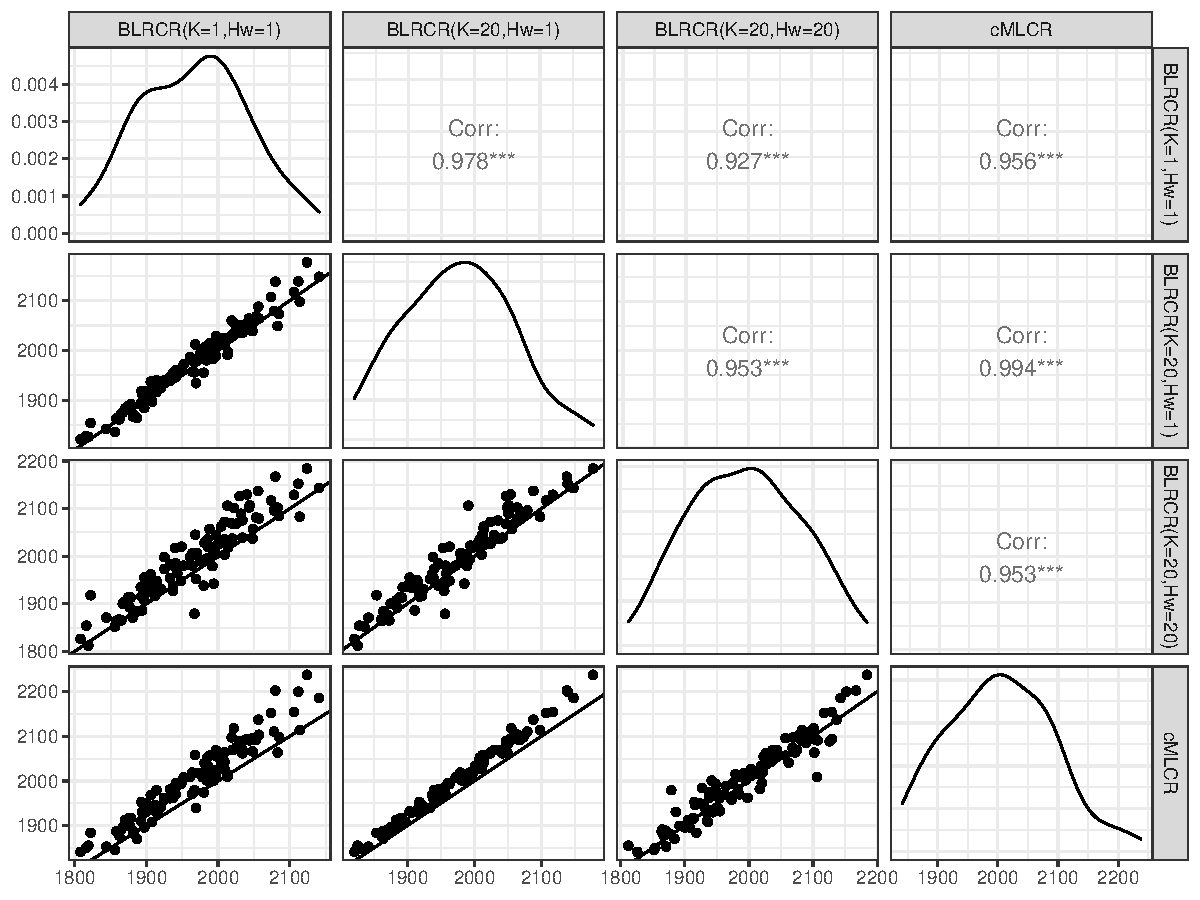
\includegraphics{dissertationmain_files/figure-latex/plotNvalues-1} 

}

\caption{\label{fig:normalx} Correlation Plot of the 100 estimates for N using BLRCR and cMLCR when simulating from two independent standard normal distributions with moderate dependency between lists and a true population size of N=2000.}\label{fig:plotNvalues}
\end{figure}

Overall, the BLRCR model is shown to be consistent. It also tends to
outperform or equally perform the other methods in terms of MSE, CI
width, and CI\(\%\).

\section{Selecting a Distribution for the Covariates}
\label{Sec:selectcovariates}

When the probability that an individual is captured at least once is
dependent upon the covariates, the observed covariate distribution will
differ from population covariate distribution. Simply using logistic
regression on the observed data would lead to biased coefficients, which
in turn would lead to bias in the population estimation. The algorithm
presented in subsection \ref{Sec:BLRCRmodel} alleviates this problem by
concatenating samples of the missing covariates with the observed data
before estimating the coefficients. Unfortunately, this presents an
additional burden on the user of specifying a distribution for the
missing covariates, \(\boldsymbol{g}(\boldsymbol{\phi})\).

\subsection{Specifying a Distribution for the Covariates}
\label{sec:normaldistributioncovariate}

If the distribution is known including parameters, then we can simply
use the aforementioned algorithm. If the distribution is known except
for the parameters, then we could specify that distribution along with
priors on the parameters. For example, \cite{royle_analysis_2009} uses a
single covariate and specifies a normal distribution with a normal
distribution prior for the mean and a gamma prior for the inverse
variance. One could take a multivariate version of this approach by
specifying,

\begin{align} 
\label{eqn:normalcovariatedistribution}
\boldsymbol{x_{i}} & \stackrel{iid}{\sim} \text{MVNormal}(\boldsymbol{\mu},\boldsymbol{\Sigma}),
\end{align}

with conjugate priors,

\begin{align}
\boldsymbol{\Sigma} \sim & \text{InvWishart}(\nu_{0},\boldsymbol{\Lambda_{0}^{-1}}) \\
\boldsymbol{\mu}|\boldsymbol{\Sigma} \sim & \text{ MVNormal}(\boldsymbol{\mu_{0}},\boldsymbol{\Sigma}/\kappa_{0})
\end{align}

This would add two additional sampling stages to the algorithm (see
\cite{gelman_bayesian_2014}):

\begin{list}{}{}
\item[1)] Sample $\boldsymbol{\Sigma}$.  Define the sufficient statistics, $\boldsymbol{\bar{x}}=\frac{1}{N}\sum_{i=1}^{N}\boldsymbol{x_{i}}$ and $\boldsymbol{S} = \sum_{i=1}^{N}(\boldsymbol{x_{i}}-\boldsymbol{\bar{x}})(\boldsymbol{x_{i}}-\boldsymbol{\bar{x}})^T$.  Then,

\begin{equation}
\boldsymbol{\Sigma} \sim \text{InvWishart}(\nu_{N},\boldsymbol{\Lambda_{N}^{-1}}),
\end{equation}

where $\nu_{N} = \nu_{0}+N$ and $\boldsymbol{\Lambda_{N}}=\boldsymbol{\Lambda_{0}}+\boldsymbol{S}+\frac{\kappa_{0}N}{\kappa_{0}+N}(\boldsymbol{\bar{x}}-\boldsymbol{\mu_{0}})(\boldsymbol{\bar{x}}-\boldsymbol{\mu_{0}})^T$.

\item[2)] Sample $\boldsymbol{\mu_k|\Sigma_k}$ for $k=1,...,K^*$.  Using the same defined terms in the previous step,

\begin{equation}
\boldsymbol{\mu}|\boldsymbol{\Sigma} \sim \text{MVNormal}(\boldsymbol{\mu_{N}},\boldsymbol{\Sigma}/\kappa_{N} ),
\end{equation}

where $\boldsymbol{\mu_{N}}=\frac{\kappa_{0}}{\kappa_{0}+N}\boldsymbol{\mu_{0}} + \frac{N}{\kappa_{0}+N}\boldsymbol{\bar{x}} $ and $\kappa_{N}=\kappa_{0}+N$.
\end{list}

Different specified distributions would require different sampling
procedures. In a supplementary document, \cite{royle_analysis_2009}
considers other types of covariate distributions and found some
variations in the inference. Unfortunately, knowing what distribution to
specify can be difficult as rarely would we know this distribution.
Deciding on a proposal distribution based upon the observed distribution
can be also dangerous or misleading as the observed distribution is a
truncation of the true distribution. Not only are the missing covariates
not missing at random but we do not even know how many are missing. As
we will shown in subsection \ref{Sec:simscovdists}, mispecifying the
distribution can lead to inaccurate estimations.

\subsection{Conditional Likelihood}

One approach to the problem is estimating the coefficients using the
conditional maximum likelihood, where the likelihood function to be
maximized is conditioned on the probability an individual is observed at
least once \citep{alho_logistic_1990,huggins_statistical_1989}. This
avoids the necessity of specifying a distribution for the covariates but
can lead to unstable results when the observed distribution of the
covariates is dissimilar to the population distribution of the
covariates \citep{tilling_capture-recapture_1999}. An article by
\cite{yee_vgam_2015} shows an easy way to implement the technique using
the \texttt{VGAM} package in \texttt{R}. The technique works in two
stages. First, use generalized linear models with a positive Bernoulli
family to estimate the the coefficients. This allows us to obtain fitted
values for the probability that each individual in the dataset is
missing. Second, use those fitted values in the Horvitz-Thompson
estimator \citep{horvitz_generalization_1952} to estimate the population
size, N. One could take a Bayesian approach to the logistic regression
and assign prior distributions to the parameters and estimate the
population in a similar way. We derive equations for finding the maximum
a posteriori (MAP) estimate in Section \ref{Sec:conditionalmaximumlike}:
Appendix A using gradient ascent.

\subsection{Nonparametric Distributions}

An alternative approach to the methods described above is to specify a
nonparametric distribution for the covariates. Using a nonparametric
method has the added consequence of increasing the complexity of the
model which may lead to additional difficulties in the mixing of the
posterior. Nevertheless, it comes with multiple benefits in allowing us
to maintain use of a full likelihood approach, continued extensibility,
and (most importantly) flexibility in the fitting of the covariates. In
this subsection, we present two methods for modeling the covariates in a
non-parametric fashion: The Dirichlet Process Mixture of Normal
Distributions and the Bayesian Bootstrap.

\subsubsection{Dirichlet Process Mixture of Normal Distributions}

The first method is to fit a Dirichlet process mixture of normal
distributions. This nonparametric approach fits a potentially infinite
number of multivariate normal distributions to the data. The following
is a description of the methodology and is adapted from
\cite{gelman_bayesian_2014}. This model introduces a latent variable,
\(z\), which is a latent parameter determining the mean and covariance
matrix from which the observed covariate, \(\boldsymbol{x_i}\), is
drawn. The generative process for each observation's covariate can then
be summarized as,

\begin{align}
\boldsymbol{x_i}|z_i \stackrel{ind}{\sim} & \text{ MVNormal}(\boldsymbol{\mu_k},\boldsymbol{\Sigma_k}) \hspace{5px} \text{for } i=1,...,N\\
z_i \stackrel{iid}{\sim} & \text{ Discrete}(\{1,2,...\},(\pi_1,\pi_2,...)) \hspace{5px} \text{for } i=1,...,N.
\end{align}

Therefore, the probability density function of the covariates can be
formally written as,

\begin{equation}
g(\boldsymbol{x}|\boldsymbol{\mu},\boldsymbol{\Sigma}) = \prod_{i=1}^N \prod_{k=1}^\infty \pi_k \text{ MVNormal}(\boldsymbol{x_i}|\boldsymbol{\mu_k},\boldsymbol{\Sigma_k}).
\end{equation}

In order to have a fully Bayesian approach, we assign priors to the
unknown parameters.

\begin{align}
\boldsymbol{\Sigma_k} \sim & \text{InvWishart}(\nu_{0},\boldsymbol{\Lambda_{0}^{-1}}) \\
\boldsymbol{\mu_k}|\boldsymbol{\Sigma_k} \sim & \text{ MVNormal}(\boldsymbol{\mu_{0}},\boldsymbol{\Sigma_k}/\kappa_{0}) \\
(\pi_1,\pi_2,...) \sim & SB(\alpha) \\
\alpha \sim & \text{ Gamma}(a_{\alpha},b_{\beta}),
\end{align}

where SB(\(\alpha\)) is the stick breaking process,
\citep{ishwaran_gibbs_2001}. While we model the number of latent classes
as infinite, we can approximate this infinite mixture problem by setting
a sufficiently large upperbound to the number of latent classes,
\(K^*\), and solving this finite-dimensional problem. The stick breaking
prior can therefore be defined as \(\pi_k = V_k \prod_{l<k}(1-V_l)\),
where \(V_1, ..., V_{K^*-1} \sim \text{Beta}(1,\alpha)\) and
\(V_{K^*}=1\). This upper bound, \(K^*\), should not be thought of as a
parameter as it should have no impact on the estimation process as long
as the value is set sufficiently large enough.

Using this generative scheme adds five additional sampling stages to the
algorithm presented in subsection \ref{Sec:BLRCRmodel}.

\begin{list}{}{}

\item[1)] Sample $z_i$ for $i=1,...,N$. The latent class label takes integer values from $1,...,K^*$.  To compute the probability of each latent class label for each $i$,

\begin{equation}
P(z_i=k) = \frac{\pi_k \text{ MVNormal}(\boldsymbol{x_i}|\boldsymbol{\mu_k},\boldsymbol{\Sigma_k})}{\sum_{l=1}^{K^*}\pi_l \text{ MVNormal}(\boldsymbol{x_i}|\boldsymbol{\mu_l},\boldsymbol{\Sigma_l})}.
\end{equation}

\item[2)] Sample $\boldsymbol{\Sigma_k}$ for $k=1,...,K^*$. Define $N_k=\sum_{i=1}1_{z_i=k}$ which is a count of the number of individuals in the population belonging to latent class, $k$.  Also, define the sufficient statistics, $\boldsymbol{\bar{x}_k}=\frac{1}{N_k}\sum_{i=1}^{N_k}\boldsymbol{x_{ik}}$ and $\boldsymbol{S_k} = \sum_{i=1}^{N_k}(\boldsymbol{x_{ik}}-\boldsymbol{\bar{x}_k})(\boldsymbol{x_{ik}}-\boldsymbol{\bar{x}_k})^T$.  Then,

\begin{equation}
\boldsymbol{\Sigma_k} \sim \text{InvWishart}(\nu_{N_k},\boldsymbol{\Lambda_{N_k}^{-1}}),
\end{equation}

where $\nu_{N_k} = \nu_{0}+N_k$ and $\boldsymbol{\Lambda_{N_k}}=\boldsymbol{\Lambda_{0}}+\boldsymbol{S_k}+\frac{\kappa_{0}N_k}{\kappa_{0}+N_k}(\boldsymbol{\bar{x}_k}-\boldsymbol{\mu_{0}})(\boldsymbol{\bar{x}_k}-\boldsymbol{\mu_{0}})^T$.

\item[3)] Sample $\boldsymbol{\mu_k|\Sigma_k}$ for $k=1,...,K^*$.  Using the same defined terms in the previous step,

\begin{equation}
\boldsymbol{\mu_k}|\boldsymbol{\Sigma_k} \sim \text{MVNormal}(\boldsymbol{\mu_{N_k}},\boldsymbol{\Sigma_k}/\kappa_{N_k} ),
\end{equation}

where $\boldsymbol{\mu_{N_k}}=\frac{\kappa_{0}}{\kappa_{0}+N_k}\boldsymbol{\mu_{0}} + \frac{N_k}{\kappa_{0}+N_k}\boldsymbol{\bar{x}_k} $ and $\kappa_{N_k}=\kappa_{0}+N_k$.

\item[4)] Sample $(\pi_1,\pi_2,...,\pi_{K^*})$ for $k=1,...,K^*$.  Begin by drawing a sample from each of the stochastic components,

\begin{equation}
 V_k \sim \text{ Beta}\left(1+N_k, \alpha+\sum_{l=k+1}^K N_l\right) \hspace{5px} \text{for } k=1,...,K^*-1.
\end{equation}

Set $V_{K*}=1$.  Then, $\pi_k = V_k\prod_{l<k}(1-V_l)$ for all $k=1,...,K^*$.

\item[5)] Sample $\alpha$.

\begin{equation}
  \alpha \sim \text{ Gamma}\left(a_\alpha + K^* -1, b_\alpha - \sum_{k}^{K^*-1}\ln(1-V_k) \right).
\end{equation}

\end{list}

It should be noted that the normal distribution specified in subsection
\ref{sec:normaldistributioncovariate} is a special case of this
specification where \(K^*=1\). We will show in section
\ref{Sec:simscovdists} that the assumption of a single normal may lead
to bias in the estimation process when the actual distribution is not
normal. Using an infinite mixture of normal distributions tends to
perform better, but still struggles when the distribution is discrete or
is far from normally distributed.

\subsubsection{The Bayesian Bootstrap}

\vspace{-10px}

An alternative approach would be to apply a discrete distribution with
support at the observed, distinct values, \(\boldsymbol{d_k}\), of the
covariates,

\begin{equation}
P(\boldsymbol{x_i}=\boldsymbol{d_k}) = \psi_k, \hspace{10px} \sum_{i=1}^K \psi_k = 1.
\end{equation}

We attach a Dirichlet prior to the probabilities, \(\psi_k\), such that

\begin{equation}
(\psi_1, ..., \psi_K) \sim Dirichlet(\alpha_1,...,\alpha_K)
\end{equation}

The posterior distribution for the \(\psi_k\) is then,

\begin{equation}
\label{eqn:bayesbootstrapposterior}
(\psi_1, ..., \psi_K|\mathcal{X}) \sim Dirichlet(\alpha_1+\sum_{i=1}^N I_{d_1}(\boldsymbol{x_i}),...,\alpha_K+\sum_{i=1}^N I_{d_K}(\boldsymbol{x_i}))
\end{equation}

where \(I_{d_k}(\boldsymbol{x_i})=1\) is an indicator function for
\(\boldsymbol{x_i} = \boldsymbol{d_i}\) and
\(I_{d_k}(\boldsymbol{x_i})=0\) otherwise.

Although we are not performing an actual bootstrapping procedure, we
refer to this modelling setup as the Bayesian Bootstrap
\citep{rubin_bayesian_1981} for a couple of reasons. First, the
construction is quite similar to the theory behind the Bayesian
Bootstrap in terms of placing a Dirichlet distribution on the observed
values in the sample. Second, this methodology samples values for the
missing observations in the same spirit as bootstrapping. Using the
\(n\) observed covariates, we sample, with replacement, \(n_0\) values
from a discrete distribution based on the observed distribution and use
these values in place of the missing covariates.

To implement this model construction for the covariates, we only need to
add one additional sampling stage to our estimation procedure. Noting
that we use all covariates, not just the observed, we draw the
probabilities, (\(\psi_1, ..., \psi_K\)) in accordance to equation
\ref{eqn:bayesbootstrapposterior}. Once the probabilities,
(\(\psi_1, ..., \psi_K\)), are drawn, the covariate distribution is
fully specified, so the rejection sampling method as displayed in
equation \ref{eqn:conditionalXmis} can be performed.

A common approximation to the Bayesian Bootstrap is to sample directly
from the empirical distribution. When
\((\alpha_1, ..., \alpha_K) = \alpha = 0\), one could skip the Dirichlet
distribution sampling stage and simply draw, with replacement, from the
current complete covariate data, \(\mathcal{X}\). While this is a good
approximation, it will have less smoothing than it's Bayesian
counterpart.

This Bayesian Bootstrap method addresses some of the potential issues in
the covariate specification, but it also introduces new issues as well.
This method provides an ``all-purpose'' solution in that it can be used
when the covariate distribution is discrete, continuous, or both.
Nevertheless, while it alleviates some of the issue with data type, no
method is truly ``all-purpose'' as any method will provide some sort of
constraint. The issues this particular model tends to have aligns
closely with those of the Bayesian Bootstrap. For example, the missing
values that are sampled only has support at values in the observed
empirical distribution. What happens if some of the potential values
that are missing do not appear in the observed distribution? This is a
concern for when the covariate distribution is discrete but a
probabilistic certainty when the distribution is continuous. This should
be a concern but as \cite{rubin_bayesian_1981} states ``serious data
analysis should always include serious consideration of model
constraints'' and that no method, even the bootstrap, is without
constraints. Furthermore, we note that the end goal is to estimate the
size of the population, so the exact modelling of the covariate
distribution is not as important as long as it does not bias the
estimation. Using the rejection sampler based on equation
\ref{eqn:conditionalXmis} combined with
\((\alpha_1, ..., \alpha_K) = \alpha = 0\), the probability of each draw
is appropriately weighted based on the probability of going unobserved.
This has similar intuition as the mechanic behind the Horvitz-Thompson
estimator in the conditional likelihood approach where each covariate
essentially gets magnified based on its estimated probability of being
missing.

\subsection{Simulations using Different Covariate Distributions}
\label{Sec:simscovdists}

EXTRA STUFF BELOW WRITTEN HERE, MAY NEED TO BE MOVED By default, we do
not use any regularization (see subsection \ref{Sec:modelselection})
unless specifically stated. For the covariate distribution, there are
three possibilities including the mixture of multivariate normal
distributions (\textbf{mixture}), the Bayesian Bootstrap
(\textbf{bootstrap}), and the approximation of the Bayesian Boostrap
that simple samples from the empirical distribution
(\textbf{empirical}). In general, the maximum number of mixture
components allowed by the mixture of multivariate normal distributions
(\(K^*\)) will be specified but is intented to be set intentially large
enough so that it does not influence the estimation. The exception would
be the case where we desire a single multivariate normal distribution
(\(K^*=1\)). Similarly, when latent intercepts are used (see subsection
\ref{Sec:condindependence}), the number of latent intercepts
(\(H_{\omega}\)) is specified.

EXTRA STUFF ABOVE WRITTEN HERE, MAY NEED TO BE MOVED

In this subsection, we examine the impact of different covariate
distributions and how they impact the BLRCR model's estimation. Recall,
the BLRCR requires the specification of a covariate distribution,
whereas the cMLCR does not. Hence, as we will see below, a
misspecification of the covariate distribution can lead to bias in the
inference. This bias will be reduced when using a more flexible
covariate distribution like the infinite mixture of normal distributions
(K=20).

\autoref{table:diffdists} presents the results of 100 simulations for
three different sets of covariate distributions. The first set of
simulations uses the two standard normal distributions seen in the
previous subsections. While the cMLCR algorithm is unbiased, all three
specifications of the BLRCR algorithm yield a lower MSE. Since the
distribution of the covariates is actually normal, it is not surprising
that the BLRCR performs well with these simulations. On the other hand,
we would expect the second set of covariates, two independent
chi-square(1) distributions, to be particularly challenging. The
chi-square distribution only has probability mass for nonnegative
values, which creates an abrupt cutoff at 0. The third set of covariates
includes two different Gamma distributions, Gamma(1,1) and Gamma(3,1).
This set of covariates cuts off abruptly on one axis at 0, but not the
other. We can therefore think of the three sets of covariates as
``normal'', ``not normal'', and ``near/approximately normal'',
respectively.

\singlespacing
\begin{table}[H]
\centering
\begin{tabular}{||r l r r r r||} 
 \hline
Distribution & Method & N$\%$ &MSE & CI Width & CI $\%$   \\ [0.5ex] 
 \hline\hline
 Normal(0,1)   & BLRCR($K=1$, $H_\omega=1$)  & 0.983   & 82.5   & 0.156   & 94.0 \\ 
 Normal(0,1)   & BLRCR($K=20$, $H_\omega=1$)    & 0.988     & 82.6     & 0.162     & 95.0 \\ 
               & BLRCR($K=20$, $H_\omega=20$)    & 0.997     & 84.9     & 0.204     & 99.0 \\
               & cMLCR       & 1.002       & 87.1      & 0.163      & 92.0 \\
               & Log Linear (BIC)  & 1.399      & 1669.3     & 0.458     & 0.0 \\ 
               & LCMCR       & 0.851       & 303.4      & 0.148      & 11.0 \\ 
               & Independent & 1.035 & 103.1& 0.157& 90.0 \\ 


 \hline
 Chi-Square(1)   & BLRCR($K=1$, $H_\omega=1$)  & 1.656   & 1383.4   & 0.950   & 0.0 \\ 
 Chi-Square(1)   & BLRCR($K=20$, $H_\omega=1$)    & 0.967     & 117.6     & 0.178     & 89.0 \\ 
                 & BLRCR($K=20$, $H_\omega=20$)    & 0.986     & 148.5     & 0.241     & 90.0 \\
               & cMLCR       & 1.008       & 104.8      & 0.183      & 92.0 \\
               & Log Linear (BIC)  & 0.892      & 973.3     & 0.217     & 6.0 \\ 
               & LCMCR       & 0.774       & 467.0      & 0.229      & 31.0 \\ 
               & Independent & 0.924 & 162.8& 0.118& 32.0 \\ 


 \hline
 Gamma(1,1)    & BLRCR($K=1$,$H_\omega=1$)  & 1.020   & 90.7   & 0.156   & 94.0 \\ 
 Gamma(3,1)    & BLRCR($K=20$, $H_\omega=1$)    & 0.986     & 63.4     & 0.132     & 99.0 \\ 
               & BLRCR($K=20$,$H_\omega=20$)    & 0.996     & 69.6     & 0.170     & 100.0 \\
               & cMLCR       & 0.999       & 55.3      & 0.123      & 96.0 \\
               & Log Linear (BIC)  & 1.247      & 1443.3     & 0.409     & 0.0 \\ 
               & LCMCR       & 0.852       & 299.3      & 0.106      & 7.0 \\ 
               & Independent & 0.863 & 276.6& 0.054& 0.0 \\ 
 \hline
\end{tabular}
\caption{Results of capture-recapture algorithms with simulations using different covariate distributions with "moderate" dependency between lists and N=2000.}
\label{table:diffdists}
\end{table}
\doublespacing

As we saw in the previous section, the BLRCR algorithm handles the
normally distributed covariates well. For the chi-square distributed
covariates, using a single multivariate normal for the covariates
results in poor performance with with an approximate bias of 1.656\(\%\)
of \(N\) when \(N=2000\). Even though the covariates are not normally
distributed, modeling them as a mixture of normal distributions results
in a substantial reduction in the bias for \(N\).
\autoref{fig:covariatedists} illustrates why this may be the case
through a partial plotting of the simulated covariates. In all plots,
the black dots represent the individuals that are captured at least once
in a list. The blue dots represent the individuals that are missing. In
the first and second plot in each row, the individuals that are missing
are simulated using the BLRCR(\(K=1\), \(H_\omega=1\)) and
BLRCR(\(K=20\), \(H_\omega=1\)) algorithms, respectively. The third
panel shows the true missing individuals that are unknown to the
algorithm. With the chi-square distribution, there is no good way to fit
a single normal variable that well represents the space. As a result,
many missing covariates are populated into low probability density areas
resulting in an overestimate of the missing covariates. On the other
hand, the BLRCR(\(K=20\), \(H_\omega=1\)) with it's less rigid covariate
assumption, populates the space much better.

\begin{figure}[H]

{\centering 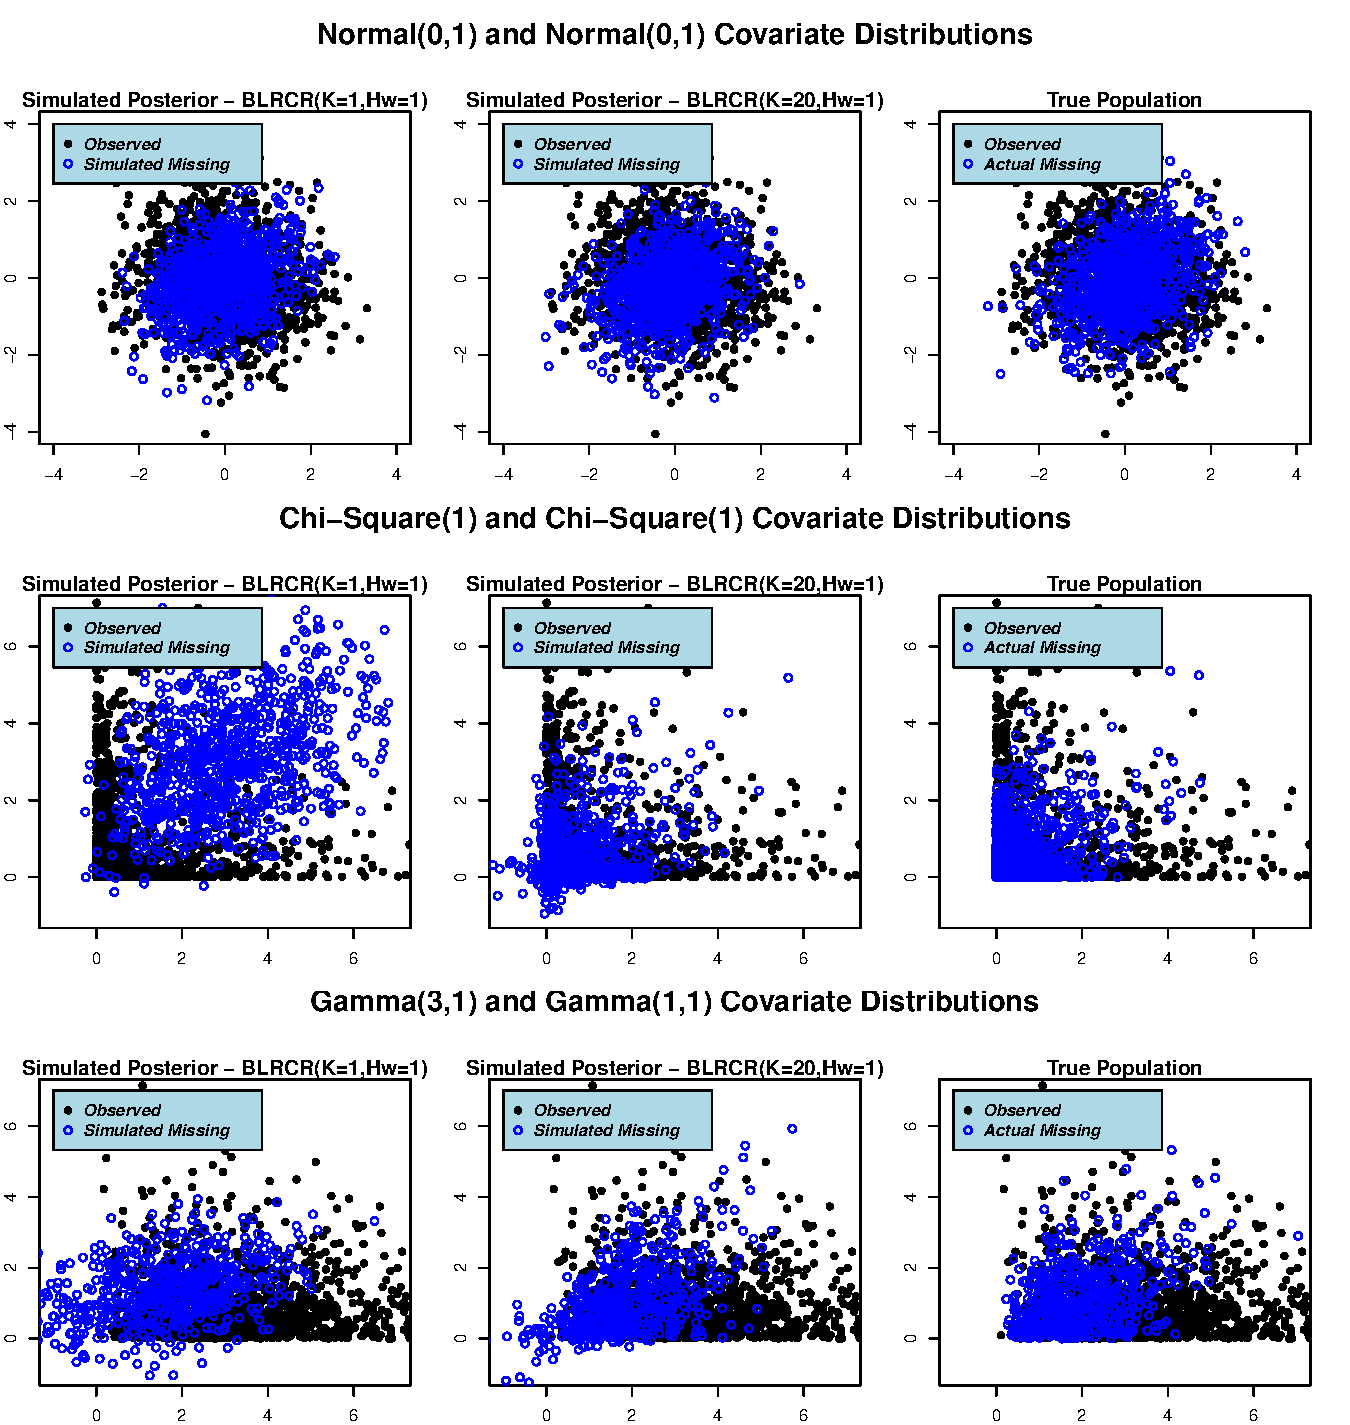
\includegraphics{dissertationmain_files/figure-latex/posteriornormalplots-1} 

}

\caption{\label{fig:covariatedists}Posterior Distribution of X when simulating various covariate distributions with moderate dependency between lists and N=2000.}\label{fig:posteriornormalplots}
\end{figure}

The parameters of the covariate distribution are sampled based on
augmented covariates, not just the observed covariates. This results in
uncertainty regarding the ability for the algorithm to correctly
identify the covariate distribution. To put the algorithm to the test,
we simulate an example with a mixture of three multivariate normal
distributions. We use a population of size 2000 and the ``moderate''
coefficients. The results of the 100 simulations can be found in
\autoref{table:mixdist}. Despite on average nearly 50\(\%\) of
observations being missing, the algorithm when allowing for up to
\(K=20\) mixture normal distributions performs well. Of course, the
cMLCR outperforms the algorithm in terms of MSE, but the BLRCR (without
also trying to account for heterogeneity) is more precise with a smaller
average credible interal width.

\singlespacing
\begin{table}[H]
\centering
\begin{tabular}{||r l r r r r||} 
 \hline
Distribution & Method & N$\%$ &MSE & CI Width & CI $\%$   \\ [0.5ex] 
 \hline\hline
 Mixture Normal& BLRCR($K=1$,$H_\omega=1$)  & 0.931   & 160.1   & 0.163   & 67.0 \\ 
               & BLRCR($K=20$,$H_\omega=1$)    & 0.977     & 97.9     & 0.183     & 96.0 \\ 
               & BLRCR($K=20$,$H_\omega=20$)    & 0.989     & 96.3     & 0.228     & 99.0 \\  
               & cMLCR       & 1.003       & 90.3      & 0.191      & 96.0 \\
               & Log Linear (BIC)  & 1.331      & 1331.4     & 0.427     & 0.0 \\ 
               & LCMCR       & 0.851       & 305.5      & 0.218      & 25.0 \\ 
               & Independent & 1.007 & 80.0& 0.173& 96.0 \\ 

 \hline
\end{tabular}
\caption{Results of capture-recapture algorithms with simulations using different covariate distributions with "moderate" dependency between lists.}
\label{table:mixdist}
\end{table}
\doublespacing

A look at the simulated posterior of the covariates in
\autoref{fig:mixx} shows once again the benefits of using the mixture of
normal distributions. Using a single multivariate normal results in an
imputation of covariates in low probability mass spaces, especially
between the lower two mixtures. When a mixture of normal distributions
is used, the imputation of the covariates is fairly consistent with the
true distribution.

\begin{figure}[H]

{\centering 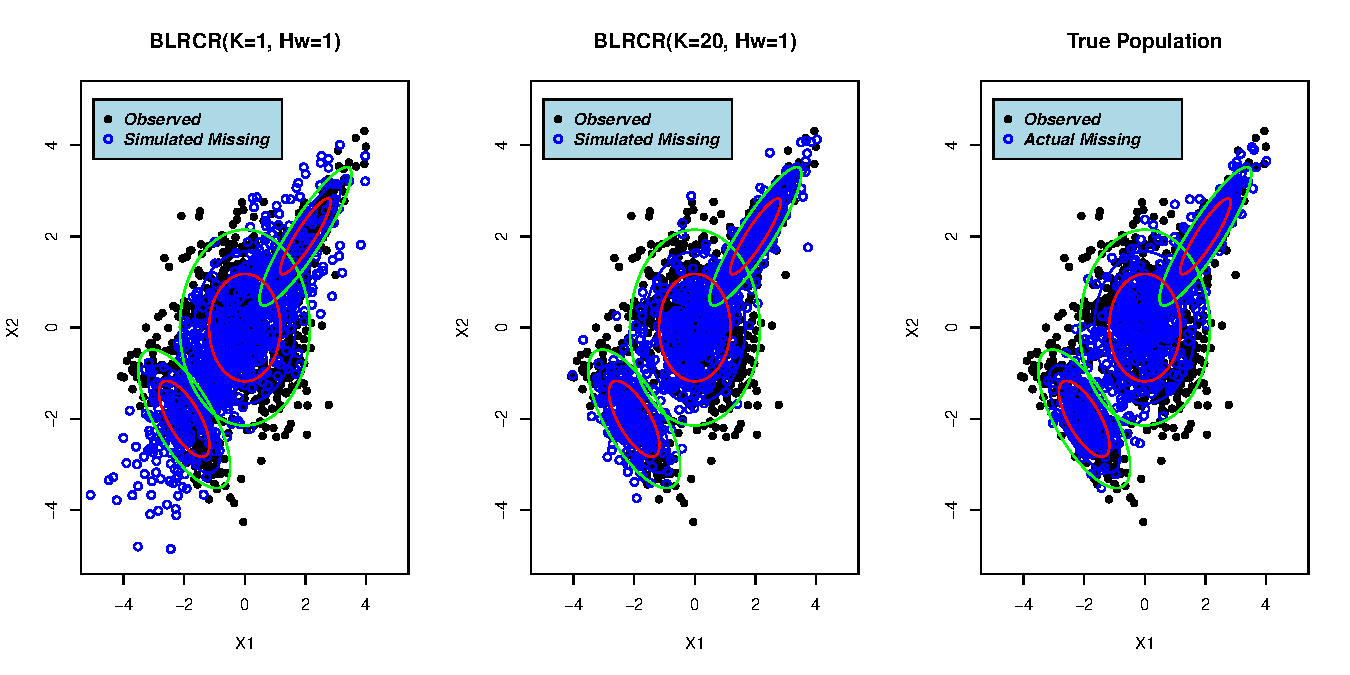
\includegraphics{dissertationmain_files/figure-latex/posteriormixtureplots-1} 

}

\caption{\label{fig:mixx}Posterior Distribution of the missing X values using algorithm SP-BLRCR.}\label{fig:posteriormixtureplots}
\end{figure}

From this subsection, we saw that depending on the level of the
covariate distribution misspecification, the BLRCR model may perform
poorly. However, using a non-parametric distribution like the mixture of
normal distributions considerably reduced the bias.

\section{Conditional Independence and Unobserved Heterogeneity}
\label{Sec:condindependence}

The model construction of subsection \ref{Sec:BLRCRmodel} assumes
conditional independence based on the covariates. In other words, given
the information provided by the covariates, the probability of capture
on one list is unaffected by another list. If the assumption does not
hold, it may lead to biased parameter estimates. One reason the
conditional independence may be violated is because the capture
probabilities upon a list are directly related to the probability of
being on another list, i.e., the assumption of list dependency. This may
occur if, for example, one list uses another list as a reference or data
is shared between various documentation projects
\citep{manrique-vallier_capture-recapture_2020}. This would lead to
heavy positive dependence between these two lists. While this is a
serious issue, we assume the lists used in the analysis are collected
independently.

A second reason conditional independence may be violated is that
underlying heterogeneity exists within the population that is not fully
accounted for by covariates. Recall, the example cited in subsection
\ref{sec:earlyapproachlitreview} of individual heterogeneity
masquerading as list dependency in the study analyzing extrajudicial
killings during the Guatemalan Civil War \citep{ball_making_2000}.
Researchers found that people who were part of Catholic religious
communities were more likely to trust Catholic researchers with their
stories than with NGO researchers associated with the political left.
Similarly, people located in areas associated with the rebel groups were
more likely to do the opposite. If this trait is unobserved and not
taken into account, it will result in biased \(\boldsymbol{\beta_j}\)
coefficients. Further, because of the biased coefficients, the
probabilities of capture and the estimate for the population size will
be biased as well.

\subsection{Modelling the Unobserved Heterogeneity with Latent Classes}

We view the problem of unobserved heterogeneity through the lens of a
missing covariates problem. There are multiple ways one can induce
additional heterogeneity into the modelling. For example,
\cite{king_bayesian_2008} uses individual random effects following a
normal distribution, while \cite{manriquevallier_bayesian_2016} induces
heterogeneity by assigning different capture probabilities according to
latent group membership. In this subsection, we model hidden
heterogeneity also through the use of latent group membership, but
instead of each group being assigned a different probability, each group
is instead given a different value for an intercept in the linear
equation.

Define an indicator vector, \(\boldsymbol{\omega_i}\), indicating
membership to one of potentially infinite latent groups. As we saw in
subsection \ref{sec:normaldistributioncovariate} with the infinite
mixture of normal distributions, we again make use of the stick-breaking
procedure in order to avoid self-selecting the number of the classes to
uses. Hence,

\vspace{-10px}

\begin{equation}
\boldsymbol{\phi_\omega}\sim \text{SB}(\boldsymbol{\alpha_\omega})
\end{equation} \begin{equation}
\alpha_\omega \sim \text{Gamma}(a_\omega,b_\omega).
\end{equation}

An additional intercept term is added to the linear equation with the
value dependent on the individual's latent class membership. As such,
equation \ref{eqn:sigmoidfunc} then becomes,

\begin{equation}
\label{eqn:sigmoidfunclatentvariable}
\lambda_{ij}=\sigma(\boldsymbol{x_i}^T\boldsymbol{\beta_j} + \boldsymbol{\omega_i}^T\boldsymbol{\beta_\omega}) = \frac{1}{1+e^{-(\boldsymbol{x_i}^T\boldsymbol{\beta_j}+\boldsymbol{\omega_i}^T\boldsymbol{\beta_\omega}))}}.
\end{equation}

This construction leads to four new types of parameters to sample:
\(\boldsymbol{\omega_i}\), \(\alpha_\omega\),
\(\boldsymbol{\phi_\omega}\), and \(\boldsymbol{\beta_\omega}\).

\subsection{Updating the Estimation}

Since we have four new parameters: \(\boldsymbol{\omega_i}\),
\(\alpha_\omega\), \(\boldsymbol{\phi_\omega}\), and
\(\boldsymbol{\beta_\omega}\); we might expect to need just four new
sampling methods. Unfortunately, complications once again arise from the
missing covariates of the unobserved individuals. If the individual is
observed, the latent group membership, \(\boldsymbol{\omega_i}\), can be
sampled with corresponding discrete probability,

\begin{equation}
\label{eqn:latentvariableomega}
p(\boldsymbol{\omega_i}|\boldsymbol{\phi_\omega},N,\mathcal{Y},\boldsymbol{\beta},\boldsymbol{X}) \propto \phi_\omega\prod_{j=1}^J\lambda_{ij}^{y_{ij}}(1-\lambda_{ij})^{1-y_{ij}}.
\end{equation}

For the individuals that are not observed, we draw the latent class
membership during the missing covariate imputation stage. Recall,
because of the complications mentioned in subsection
\ref{sec:estimationBLRCRMCMC}, the Gibbs sampler requires \(N\) and
\(\mathcal{X}_{mis}\) to be sampled simultaneously. In order to
implement this stage, the latent class membership,
\(\boldsymbol{\omega_i}\) of each unobserved individual must be drawn
along with, presumably independently, the missing covariates,
\(\mathcal{X}_{mis}\). Whereas the distribution from which the
covariates is drawn is dependent on the covariate distribution selected
(see subsection \ref{Sec:selectcovariates}), the \(\omega_i\)'s are
drawn from the discrete distribution with probability vector
\(\boldsymbol{\phi_\omega}\).

Once again, we use a finite representation of the stick-breaking process
for estimation purposes with a sufficiently large upperbound,
\(H_\omega^*\). Under this construction, the stick-breaking process is
defined as
\((\phi_{1},\phi_{2},...,\phi_{H_\omega^*}) = V_{h} \prod_{{h'}<h}(1-V_{{h'}})\),
where
\(V_{1}, V_{2}, ..., V_{H_\omega^*-1} \sim \text{Beta}(1,\alpha_\omega)\)
and \(V_{H_\omega^*}=1\). To obtain samples from the conditional
posterior distribution, \(p(\phi_\omega|...)\), we first sample \(V_h\)
by,

\vspace{-10px}

\begin{equation}
\label{eqn:latentvariablePHIomega}
V_h \sim \text{Beta}\Big(1+N_h,\alpha_\omega + \sum_{h'=h+1}^{H^*_\omega} N_{h'}\Big),
\end{equation}

for all \(h=1,...,H_\omega^*-1\) where \(N_{h}\) is the number of
individuals belonging to each latent class. Then compute
\(\phi_{h} = V_h \prod_{{h'}<h}(1-V_{h'})\) for \(h=1,...,H^*_\omega.\)
The conditional posterior distribution, \(p(\alpha_\omega|...)\) can be
sampled by

\vspace{-10px}

\begin{equation}
\label{eqn:alphaomegacondsampling}
\alpha_\omega \sim \text{Gamma}\Big(a_\omega + H_\omega^* - 1, b_\omega - \sum_{h=1}^{H^*_\omega-1}\ln (1-V_h)\Big),
\end{equation}

Lastly, the coefficient vector of latent intercepts,
\(\boldsymbol{\beta_\omega}\), can be sampled in the same manner as the
other coefficients, \(\boldsymbol{\beta_j}\).

\subsection{Simulations with Unobserved Heterogeneity}
\label{Sec:simsunobservedheterogeneity}

The final set of simulations is to demonstrate the importance of
accounting for both the observed and unobserved heterogeneity. While the
cMLCR model has performed well in the prior sections, it has no method
of detecting unobservable heterogeneity and hence produces biased
estimation. Interestingly, a model like the LCMCR, which is designed to
account for unobservable heterogeneity, performs much better, but still
struggles as considerable information can be gained by including the
covariates. The BLRCR model when extended to include latent intercepts
(\(H_\omega>1\)) can utilize the covariates to detect the observable
heterogeneity, but also accounts for the additional unobservable
heterogeneity. As a result, it is the only model that performs well in
this subsection.

Data is simulated for three lists (J=3) with one standard normally
distributed observed covariate (H=1) and one unobserved covariate
indicating membership to a latent group with probability 0.35. The
coefficients used to simulate the data can be found in
\autoref{table:heterocoefs}. Using these coefficients induces positive
dependency between lists 1 and 2, but negative dependency between list 3
and the other two lists. If class membership were known, the list
probabilities would still be conditionally independent; however, since
these covariates are unobserved, the list probabilities are no longer
conditionally independent given the observed data.

\singlespacing
\begin{table}[H]
\centering
\begin{tabular}{||c c c c||} 
 \hline
 List ($j$) & $\beta_{0j}$ & $\beta_{1j}$ & $\beta_{\omega j}$   \\ [0.5ex] 
 \hline\hline
 1 & -2.5 &  -1.5  & 3.0 \\ 
 2 & -2.5 & -1.5  &  3.0 \\
 3 & 0.5 & -1.5  &  -3.0 \\
 \hline
\end{tabular}
\caption{Coefficients for Heterogeneity Simulated Data}
\label{table:heterocoefs}
\end{table}
\doublespacing

\autoref{table:heterodist} shows the results of 100 simulations on four
different population sizes. It becomes obvious that not accounting for
unobserved heterogeneity results in biased estimates for both the BLRCR
and cMLCR models. Recall, the truth with these simulations is there
exists two latent classes. Notice the BLRCR model with the number of
hidden classes set at \(H_\omega=2\) performs the best in terms of both
accuracy and precision. In a real setting, the number of hidden classes
would almost certainly be unknown so we set a sufficiently large value
\(H_\omega=20\). While the model doesn't perform quite as well as the
aforementioned setting, it dramatically outperforms the methods that do
not take unobserved heterogeneity into account.

For situations where observed and unobserved heterogeneity exist, we
need a method that accounts for both. It should be noted that the LCMCR
model, a methodology that doesn't use covariates, is outperforming the
methods that do but assume conditional independence. The LCMCR model is
designed to account for unobserved heterogeneity, and since the
unobserved heterogeneity plays a substantial role in the capture
probability for these simulations, it performs reasonably well. Of
course, as we saw in the previous subsections' simulations, the LCMCR
does not perform as well as the other methods when most of the
heterogeneity can be explained by the covariates.

To further explore the effects of hidden heterogeneity and its
detectability, we ran 100 simulations with different coefficients and
group percentages. Using the same coefficients in
\autoref{table:heterocoefs}, but adjusting the absolute value of the
coefficients, \(\beta_{\omega_j}\), we created scenarious that depict
different strength levels of heterogeneity. Trivially, if the
coefficient is 0, there is no unobserved heterogeneity in the capture
probabilities. In this situation the algorithm is simply detecting noise
that it is mistaking for heterogeneity. On the other hand, when the
absolute value of the \(\beta_{\omega j}\) coefficients are set to 5,
there is very strong heterogeneity in the capture probabilities for the
two groups. The top plot in \autoref{fig:heterogeneitydiff} shows the
mean square error (MSE) of the 100 simulations' posterior median of
\(N\). A close examination of the plot reveals an overall decrease in
the MSE as the heterogeneity strengthens. This is not surprising as the
model is attempting to account for heterogeneity, but if it cannot
detect the heterogeneity, it will induce bias. When the heterogeneity is
stronger, the model is more likely to detect this heterogeneity and
account for it properly.

\singlespacing
\begin{table}[H]
\centering
\begin{tabular}{||r l r r r r||} 
 \hline
N & Method & N$\%$ &MSE & CI Width & CI $\%$   \\ [0.5ex] 
 \hline\hline



 1000          & BLRCR($K=1$, $H_\omega=1$)  & 1.192   & 209.0   & 0.386   & 25.0 \\ 
               & BLRCR($K=20$, $H_\omega=1$)    & 1.192     & 207.6     & 0.382     & 24.0 \\ 
               & BLRCR($K=20$, $H_\omega=2$)    & 0.997     & 57.5     & 0.334     & 100.0 \\ 
               & BLRCR($K=20$, $H_\omega=20$)    & 0.986     & 67.9     & 0.385     & 100.0 \\ 
               & cMLCR       & 1.231       & 250.8      & 0.390      & 25.0 \\
               & Log Linear (BIC)  & 1.048      & 94.7     & 0.199     & 64.0 \\ 
               & LCMCR       & 0.851       & 156.0      & 0.414      & 93.0 \\ 
               & Independent & 0.875 & 128.2& 0.095& 1.0 \\ 

 \hline
 


 2000          & BLRCR($K=1$, $H_\omega=1$)  & 1.210   & 438.8   & 0.302   & 1.0 \\ 
               & BLRCR($K=20$, $H_\omega=1$)    & 1.205     & 428.4     & 0.295     & 1.0 \\
               & BLRCR($K=20$, $H_\omega=2$)    & 1.005     & 115.4     & 0.278     & 99.0 \\
               & BLRCR($K=20$, $H_\omega=20$)    & 0.994     & 130.0     & 0.316     & 98.0 \\ 
               & cMLCR       & 1.225       & 469.9      & 0.274      & 1.0 \\
               & Log Linear (BIC)  & 1.022      & 182.7     & 0.144     & 44.0 \\ 
               & LCMCR       & 0.858       & 301.0      & 0.388      & 93.0 \\ 
               & Independent & 0.872 & 259.3& 0.067& 0.0 \\ 

 \hline
 


 5000          & BLRCR($K=1$, $H_\omega=1$)  & 1.229   & 1161.6   & 0.223   & 0.0 \\ 
               & BLRCR($K=20$, $H_\omega=1$)    & 1.222     & 1127.8     & 0.219     & 0.0 \\ 
               & BLRCR($K=20$, $H_\omega=2$)    & 1.010     & 217.2     & 0.208     & 100.0 \\
               & BLRCR($K=20$, $H_\omega=20$)    & 1.005     & 236.1     & 0.235     & 100.0 \\ 
               & cMLCR       & 1.230       & 1165.8      & 0.173      & 0.0 \\
               & Log Linear (BIC)  & 0.954      & 478.7     & 0.108     & 22.0 \\ 
               & LCMCR       & 0.869       & 700.0      & 0.340      & 85.0 \\ 
               & Independent & 0.874 & 630.3& 0.042& 0.0 \\ 

 \hline
 


 10000          & BLRCR($K=1$, $H_\omega=1$)  & 1.224   & 2261.2   & 0.183   & 0.0 \\ 
               & BLRCR($K=20$, $H_\omega=1$)    & 1.219     & 2202.3     & 0.180     & 0.0 \\ 
               & BLRCR($K=20$, $H_\omega=2$)    & 1.005     & 359.1     & 0.164     & 99.0 \\
               & BLRCR($K=20$, $H_\omega=20$)    & 1.008     & 406.3     & 0.191     & 98.0 \\ 
               & cMLCR       & 1.221       & 2230.8      & 0.120      & 0.0 \\
               & Log Linear (BIC)  & 0.917      & 935.4     & 0.088     & 5.0 \\ 
               & LCMCR       & 0.869       & 1426.7      & 0.322      & 77.0 \\ 
               & Independent & 0.872 & 1277.3& 0.030& 0.0 \\ 

 \hline
\end{tabular}
\caption{Results of 100 capture-recapture simulations per algorithm using a standard normal distribution distribution for the known covariate and 0.35 probability of belonging to the latent class.}
\label{table:heterodist}
\end{table}
\doublespacing

\begin{figure}[H]

{\centering 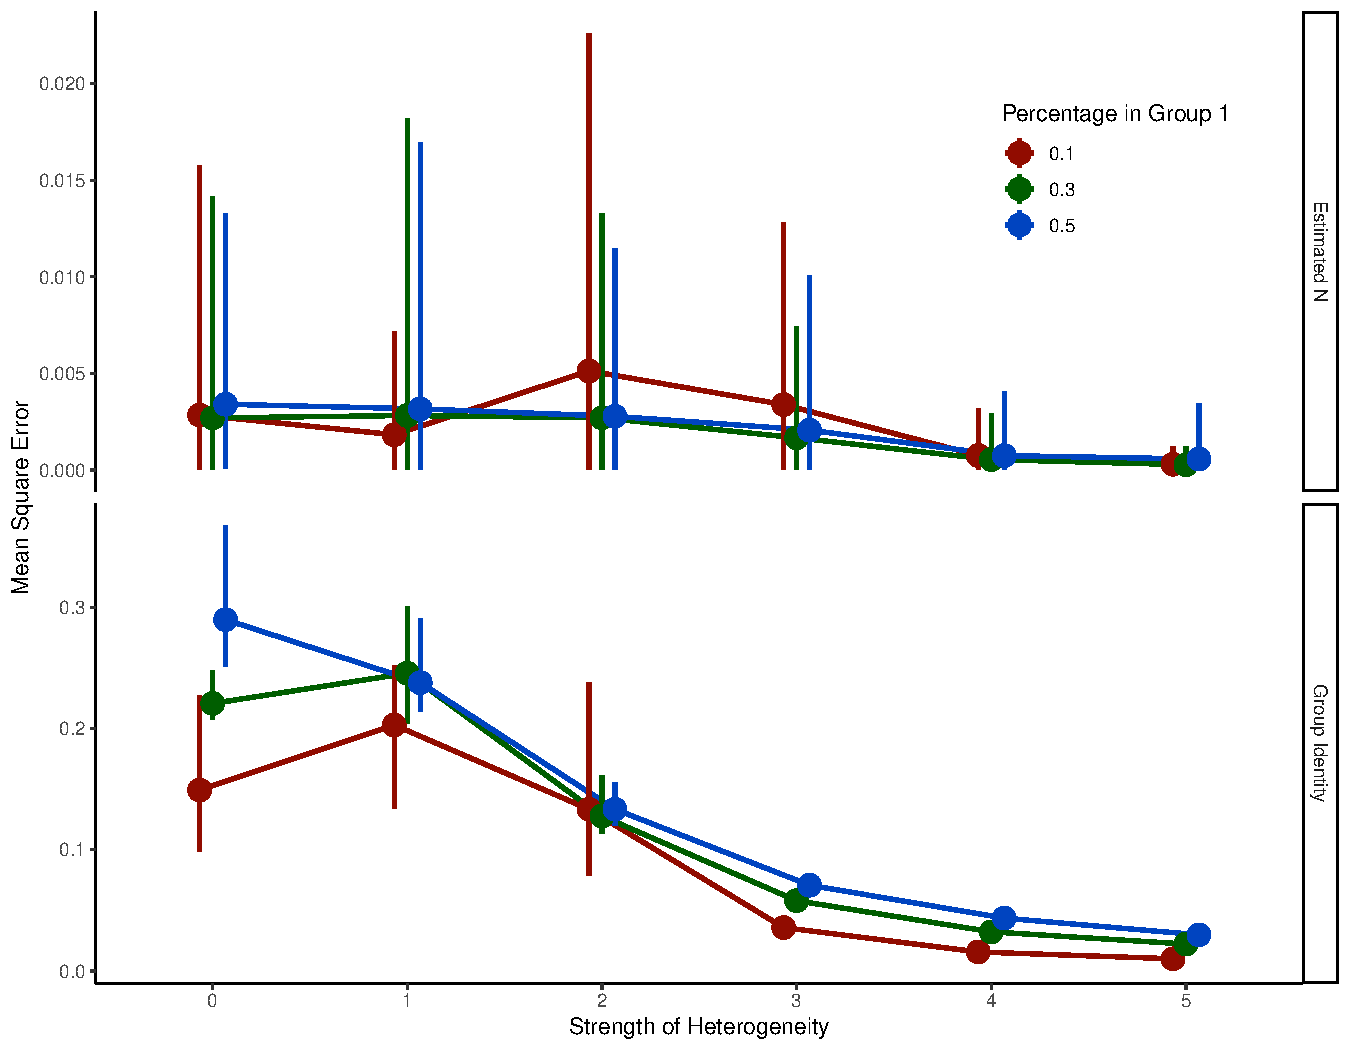
\includegraphics{dissertationmain_files/figure-latex/heterogeneitydiff-1} 

}

\caption{\label{fig:strengthheterogeneitydiff}Effect of Strength of Heterogeneity on the Mean Square Error}\label{fig:heterogeneitydiff}
\end{figure}

The bottom plot in \autoref{fig:heterogeneitydiff} shows the MSE of the
average posterior group identifier for the observed data. In other
words, if the first observation actually belongs to the hidden group,
\(\omega_1\)=1, then we find the average number of times the algorithm
placed the observation in the first group, \(\bar{\omega}_1\). In the
binary case, \(H_\omega=2\), the MSE can be computed as

\begin{equation}
MSE = \frac{1}{n}\sum_{i=1}^n (\bar{\omega}_{i} - \omega_i)^2.
\end{equation}

As the heterogeneity strengthens, the detectability of the unobserved
groupings increases and the MSE drops considerably. In the case where
the absolute value of \(\beta_{\omega j}\) is set to 5, in many of the
simulations between 90 and 95\(\%\) of the observations are detected
correctly in over 90\(\%\) of posterior samples.

Unobserved heterogeneity creates a trade off. On one hand, if the
unobserved heterogeneity is weak, there will be relatively little bias
in \(N\); however, the ability to detect this heterogeneity decreases as
well. On the other hand, When the unobserved heterogeneity is strong,
the bias in \(N\) will be relatively larger, but the ability to detect
and properly account for this heterogeneity increases.

\section{Model Selection}
\label{Sec:modelselection}

The methodology described in the previous sections assumes the
practitioner knows exactly how the covariates impact the probability of
each individual going undetected on a given list. The key to the
successful estimation of the population size relies on the proper and
accurate sampling of the coefficients in the logistic regression, or at
a minimum, these cofficients must lead to a correct estimate of the
overall probability of an individual being missing. Hence, one must
carefully select which covariates to use, how to use these covariates,
and whether there are any interactions that may play an important role
in this process. While it may be beneficial to rely on domain knowledge
of the population to make these determinations, this may not be
sufficient so it is desirable to take a statistical approach to this
problem.

\subsection{Model Comparison via the Bayes Factor}

Perhaps the most ubiquitous approach to model selection in a Bayesian
setting is through the computation of the Bayes Factor. This approach of
model comparison has a lot of similarities with the problem of
hypothesis testing. Suppose there is a null and alternative model,
\(\mathcal{M}_0\) and \(\mathcal{M}_1\), respectively. With the standard
frequentist approach, the practitioner computes the the probability of
observing the data given the null model, the p-value, and chooses to
accept or reject the null model based on some arbitrary threshold,
typically based on controlling for Type I error. On the other hand,
using a Bayesian approach
\citep{jeffreys_tests_1935,jeffreys_theory_1967}, we compare two
hypotheses or models by directly computing the probability of each model
given the data through the posterior probabilities. This means, unlike
frequentist hypothesis testing, there is no need to distinguish between
which model is the null and which is the alternative.

For the BLRCR model, the posterior probability of \(\mathcal{M}_1\)
given the observed data is written as

\vspace{-20px}

\begin{align}
p(\mathcal{M}_1|\mathcal{Y}_{obs},\mathcal{X}_{obs}) = \frac{p(\mathcal{Y}_{obs},\mathcal{X}_{obs}|\mathcal{M}_1)p(\mathcal{M}_1)}{p(\mathcal{Y}_{obs},\mathcal{X}_{obs})}.
\end{align}

\vspace{-20px}

Next, we calculate the posterior odds ratio between \(\mathcal{M}_1\)
and \(\mathcal{M}_0\) as

\vspace{-20px}

\begin{align}
\frac{p(\mathcal{M}_1|\mathcal{Y}_{obs},\mathcal{X}_{obs})}{p(\mathcal{M}_0|\mathcal{Y}_{obs},\mathcal{X}_{obs})} = 
\frac{p(\mathcal{Y}_{obs},\mathcal{X}_{obs}|\mathcal{M}_0)p(\mathcal{M}_0)}{p(\mathcal{Y}_{obs},\mathcal{X}_{obs}|\mathcal{M}_1)p(\mathcal{M}_1)}.
\end{align} \vspace{-20px}

If we do not a priori favor one model over another, such that
\(p(\mathcal{M}_0)=p(\mathcal{M}_1)\), then the posterior odds ratio is
equal to what is known as the Bayes Factor,

\vspace{-20px}

\begin{align}
\label{eqn:bayesfactorformula}
BF_{10} & = \frac{p(\mathcal{Y}_{obs},\mathcal{X}_{obs}|\mathcal{M}_1)}{p(\mathcal{Y}_{obs},\mathcal{X}_{obs}|\mathcal{M}_0)}.
\end{align} \vspace{-20px}

where values greater than 1 would suggest \(\mathcal{M}_1\), and values
less than 1 would suggest \(\mathcal{M}_0\) as the better fit.

Calculation of the Bayes Factor is often difficult or intractable as it
is the ratio of the marginal likelihoods of the two models. Given a
specific model, \(\mathcal{M}_i\), The marginal likelihood is the
probability of the data integrated across all values of the parameters,

\vspace{-20px}

\begin{align}
\label{eqn:marginallikelihoodBF}
p(\mathcal{Y}_{obs},\mathcal{X}_{obs}|\mathcal{M}_i) & = \int p(\mathcal{Y}_{obs},\mathcal{X}_{obs}|\boldsymbol{\theta},\mathcal{M}_i)p(\boldsymbol{\theta}|\mathcal{M}_i) d\boldsymbol{\theta}.
\end{align} \vspace{-20px}

This is the the denominator in the calculation of the posterior
distribution assuming a fixed model (ignore the \(\mathcal{M}_i\)).
Because this is just the normalizing constant on the posterior density
and because of the complexity of its calculation, the calculation of the
marginal likelihood is often avoided by taking advantage of
posterior/prior conjugacy or normalization in the discrete case.

Without the ability to solve Equation \ref{eqn:marginallikelihoodBF}
analytically, we must rely on an approximate solution. Perhaps the
simplest solution is to recognize Equation
\ref{eqn:marginallikelihoodBF} can be written as the expected value of
the likelihood under the prior distribution. As such, a simple
application of the Law of Large numbers, leads to the estimator,

\vspace{-20px}

\begin{align}
\label{eqn:priorapproxBF}
\hat{p}_1(\mathcal{Y}_{obs},\mathcal{X}_{obs}|\mathcal{M}_i) & =\frac{1}{G}\sum_{g=1}^G p(\mathcal{Y}_{obs},\mathcal{X}_{obs}|\boldsymbol{\theta}^{(g)},\mathcal{M}_i),
\end{align} \vspace{-20px}

where \(G\) is the number of samples and \(\boldsymbol{\theta}^{(g)}\)
are the sampled parameter values from the \textbf{prior} distribution.
While this estimator is simple and easy to implement, it converges
slowly when the prior and posterior are significantly different, which
is often the case when using non-informative priors. Many of the prior
samples will produce negligibly small likelihood values, leading to a
large variance in the estimator. One solution to improve this
integration is to use importance sampling
\cite{kass_bayes_1995,robert_computational_2009}, but leads to the
additional hardship of selecting a proper importance sampling function.
Furthermore, this method requires sampling from the prior which creates
additional difficulties when using an improper prior such as the prior
for \(N\) as with the BLRCR.

Instead of using the prior distribution, \cite{newton_approximate_1994}
showed that the harmonic mean can be used to approximate the marginal
likelihood using posterior samples,

\vspace{-20px}

\begin{align}
\label{eqn:harmonicmeanBF}
\hat{p}_2(\mathcal{Y}_{obs},\mathcal{X}_{obs}|\mathcal{M}_i) & = \left[\frac{1}{G}\sum_{g=1}^G \frac{1}{p(\mathcal{Y}_{obs},\mathcal{X}_{obs}|\boldsymbol{\theta}^{(g)},\mathcal{M}_i)}\right]^{-1},
\end{align} \vspace{-20px}

where \(\boldsymbol{\theta}^{(g)}\) are the sampled parameter values
from the \textbf{posterior} distribution. Unfortunately, this estimator
tends to not work well with results being unstable and the estimator
having infinite variance
\citep{neal_contribution_1994,robert_computational_2009}. To improve
this estimator, \cite{newton_approximate_1994} present additional
estimators using mixtures from the prior and posterior. Alternatively,
\cite{gelfand_bayesian_1994} derives an estimator in the context of
importance sampling where the posterior distribution is selected as the
importance sampling density.

\vspace{-20px}

\begin{align}
\label{eqn:harmonicmeanimportanceBFderivation}
\nonumber E_{p(\boldsymbol{\theta}|\mathcal{Y}_{obs},\mathcal{X}_{obs})}\left[\frac{\psi(\boldsymbol{\theta})}{p(\boldsymbol{\theta})p(\mathcal{Y}_{obs},\mathcal{X}_{obs}|\boldsymbol{\theta})}\right] & =\int \frac{\psi(\boldsymbol{\theta})}{p(\boldsymbol{\theta})p(\mathcal{Y}_{obs},\mathcal{X}_{obs}|\boldsymbol{\theta})}\cdot p(\boldsymbol{\theta}|\mathcal{Y}_{obs},\mathcal{X}_{obs})d\boldsymbol{\theta}\\
\nonumber & =\int \frac{\psi(\boldsymbol{\theta})}{p(\boldsymbol{\theta})p(\mathcal{Y}_{obs},\mathcal{X}_{obs}|\boldsymbol{\theta})}\cdot\frac{p(\boldsymbol{\theta})p(\mathcal{Y}_{obs},\mathcal{X}_{obs}|\boldsymbol{\theta})}{p(\mathcal{Y}_{obs},\mathcal{X}_{obs})}d\boldsymbol{\theta}\\
\nonumber & =\frac{1}{p(\mathcal{Y}_{obs},\mathcal{X}_{obs})} \int \psi(\boldsymbol{\theta}) d\boldsymbol{\theta}\\
& =\frac{1}{p(\mathcal{Y}_{obs},\mathcal{X}_{obs})}
\end{align} \vspace{-20px}

where \(\psi(\boldsymbol{\theta})\) can be any proper density. Hence a
consistent estimator for the marginal likelihood is

\vspace{-20px}

\begin{align}
\label{eqn:harmonicmeanimportanceBF}
\hat{p}_3(\mathcal{Y}_{obs},\mathcal{X}_{obs}|\mathcal{M}_i) & = \left[\frac{1}{G}\sum_{g=1}^G \frac{\psi(\boldsymbol{\theta}^{(g)})}{p(\boldsymbol{\theta}^{(g)}|\mathcal{M}_i)p(\mathcal{Y}_{obs},\mathcal{X}_{obs}|\boldsymbol{\theta}^{(g)},\mathcal{M}_i)}\right]^{-1}.
\end{align} \vspace{-20px}

Notice that if we set
\(\psi(\boldsymbol{\theta}^{(g)}) = p(\boldsymbol{\theta}^{(g)})\), we
have the original harmonic mean estimator,
\(\hat{p}_2(\mathcal{Y}_{obs},\mathcal{X}_{obs}|\mathcal{M}_i)\). While
any density can be selected, we need a density with lighter tails than
\(p(\boldsymbol{\theta}^{(g)}|\mathcal{M}_i)p(\mathcal{Y}_{obs},\mathcal{X}_{obs}|\boldsymbol{\theta}^{(g)},\mathcal{M}_i)\)
in order to improve the original estimator and achieve finite variance
\citep{robert_computational_2009}. Potential candidate densities that
may work include asymptotic densities around the maximum likelihood
values or kernel approximations. For example, in the case of Probit
regression, \cite{marin_importance_2018} found success using the normal
density with mean and covariance equal to the maximum likelihood
estimate.

This subsection provides a handful of methods for computing the Bayes
Factor for the BLRCR model, but there are several potential issues
making the above procedures impossible or at best questionable to
implement. For starters, the use of improper priors on \(N\) means the
Bayes Factors should certainly not be interpreted literally as the
actual value is off by an arbitrary constant. Second, the
multi-dimensionality of the problem leads to issues of converge with
even the largest of chains. Nevertheless, we will see in {[}INSERT
SIMULATION SUBSECTION{]} that the Bayes Factor computations above lead
us to the correct implementation more often than not.

Our focus is on the methods that utilize samples from the posterior
distribution since the algorithm provided in subsection
\ref{sec:estimationBLRCRMCMC} utilizes a MCMC method. Further work could
be done on methods that use samples from the prior like the estimator,
\(\hat{p}_1(\mathcal{Y}_{obs},\mathcal{X}_{obs}|\mathcal{M}_i)\). In
addition, other approaches such as asymptotic approximations like
Laplace's Method or exploiting functional equalities
\cite{chib_marginal_1995} may prove promising as well. While we leave
this to future research, we believe a more promising approach may be
through the use of regression regularization.

\subsection{Regularization and Prior Specifications}

We propose a different approach to model selection via the Bayes factor
by instead narrowing in on the portion of the methodology that samples
the logistic regression coefficients. While the various subsections have
added stages to the BLRCR sampler to accommodate various complications,
the sampling stages can be summarized into two basic groupings as
presented in subsection \ref{sec:estimationBLRCRMCMC}. The first
grouping of sampling stages are used to augment the missing data by
first sampling the size of the data, \(N\), and then sampling the
missing covariates, \(\mathcal{X}_{mis}\). The second grouping of
sampling stages then samples the probability an individual goes missing
through a deterministic function of the sampled logistic regression
coefficients, \(\boldsymbol{\beta}\). Under this framework, taking a
sample of regression coefficients using the augmented data is no
different than taking a sample of regression coefficients from a dataset
that is static. Hence, we can narrow our focus to finding the correct
fitting for the linear component of our logistic regression.

By narrowing our focus to the regression coefficients, we can include
all potential variables (including transformations and interactions)
with the purported threat of overfitting. There are multiple ways to
overcome the problem with overfitting. A typical way seen especially in
the data science community is through cross validation using training
and testing sets. This is not a feasible approach for the
capture-recapture problem, as the number of observed captures, plays a
crucial rule in the estimation process. Theoretically, there may be ways
around this by estimating random subpopulation sizes, but as is typical
with these approaches, less data being used for estimation leads to more
uncertainty especially in the face of sparsity. As a result, we suggest
implementing regularized regression, which in a Bayesian context, is
through different types of priors.

{[}MENTION HORSESHOE and SLAB/SPIKE PRIOR HERE ALONG WITH PAPERS FOR
IMPLEMENTING, note that using normal priors is a form of regularization,
i.e.~ridge regression{]}

While regularization has its shortcomings, using these different priors
avoids many of the complications that can arise with the computation of
the Bayes Factor. Also, when the number of model comparisons is large,
computing the Bayes Factor requires posterior samples from each of the
candidate models, whereas with regularization, only one MCMC chain is
required.

\newpage
\section{Example 1 (probably superhero)}
\label{Sec:example1}

\newpage
\section{Example 2 (find something real even if we don't know the answer)}
\label{Sec:example2}

\newpage

\section{Conclusion}
\label{Sec:Conclusion}

The objective of this dissertation project is to develop a Bayesian
capture-recapture (CR) method that can utilize covariate information to
understand the heterogeneity between individuals. Presented in this
proposal is a framework for modelling capture-recapture with covariates.
Specifically, we develop the Bayesian Logistic Regression Capture
Recapture (BLRCR) that utilizes the covariate information directly in
estimating individual capture rates. Further, we account for unobserved
heterogeneity with the use of latent classes. This model is solved using
an MCMC algorithm to approximate the posterior distribution of our
population size, \(N\). I propose three primary areas of interest that
will be addressed as the focus of the dissertation: unobserved
heterogeneity, modelling the covariate distribution, and covariate
selection.

\subsection{Unobserved Heterogeneity}

This extension concerns the issue of unobserved heterogeneity described
in subsection \ref{Sec:condindependence}. To account for this
heterogeneity, the algorithm detects latent groups and applies different
intercepts in the linear term that defines the capture probability.
Currently the number of latent classes is fixed and must be selected by
the practitioner. An extension would be to include some method for
determining the number of latent classes to include. While it may be
reasonable in some cases to know the number of latent classes, an
obvious approach would be to incorporate a stick-breaking prior on the
number of latent classes.

\subsection{Modelling the Covariate Distribution}

A requirement of the algorithm is the necessity of specifying a
distribution for the missing covariates, discussed in subsection
\ref{Sec:selectcovariates}. Typically this distribution is unknown so
utilizing a distribution that is fairly flexible is ideal. In this
proposal, we implemented the non-parametric approach of using an
infinite mixture of normals with membership determiend through a
stick-breaking process (and additionally a single multivariate normal
which is a special case). While the infinite mixture of normal
distributions tends to perform well when the distribution is at least
somewhat normal, it struggles when presented with certain non-normal
distributions. Alternatively, I propose using Dirichlet process mixtures
as described in \cite{gelman_bayesian_2014}. A sufficiently large
concentration parameter, \(\alpha \rightarrow \infty\), would be in
essence the same thing as the empirical distribution.

\subsection{Covariate Selection}

If many covariates are present, we need a method for determining which
covariates should be used while also considering interaction effects.
Along these same lines, we need to consider how a variable affects the
capture probability as some sort of transformation may be required. We
suggest three possible routes including model averaging, variable
selection through priors, or even post-hoc analysis like computing the
Bayes factor.

\newpage

\section{Appendix A: Conditional Maximum Likelihood Estimation}

\label{Sec:conditionalmaximumlike}

Instead of using the full likelihood we replace it with the conditional
likelihood, conditioned on each individual being observed once.

\begin{align}
\nonumber p(\mathcal{Y}|N,\boldsymbol{\beta},\mathcal{X}_{obs},\mathcal{X}_{mis};\boldsymbol{y}\ne \boldsymbol{0}) = & \frac{p(\mathcal{Y}|N,\boldsymbol{\beta},\mathcal{X}_{obs},\mathcal{X}_{mis})}{P(\boldsymbol{y}\ne \boldsymbol{0})} \\
= & \prod_{i=1}^N \frac{\prod_{j=1}^J \lambda_{ij}^{y_{ij}}(1-\lambda_{ij})^{1-y_{ij}}}{1-\prod_{j=1}^J(1-\lambda_{ij})}
\end{align}

The posterior distribution can therefore be written as

\begin{align}
\label{eqn:condposteriorderivevalues}
\nonumber p(N,\boldsymbol{\beta},\mathcal{X}_{mis}|\mathcal{Y},\mathcal{X}_{obs}) \propto &  \left[\prod_{i=1}^N \frac{\prod_{j=1}^J \lambda_{ij}^{y_{ij}}(1-\lambda_{ij})^{1-y_{ij}}}{1-\prod_{j=1}^J(1-\lambda_{ij})} \right] \times \left[ \prod_{i=1}^N \boldsymbol{g}(\boldsymbol{\theta_h}) \right] \times  \left[\frac{1}{N}\right] \\
\times & \left[ \prod_{j=1}^J \left(\frac{1}{2\pi}\right)^{H/2}|B|^{-1/2}e^{-\frac{1}{2}(\boldsymbol{b}-\boldsymbol{\beta_j})^T\boldsymbol{B}^{-1}(\boldsymbol{b}-\boldsymbol{\beta_j})}\right].
\end{align}

Instead of computing a MCMC sampler, we will instead compute the Maximum
a posteriori (MAP) estimate for the coefficients,
\(\boldsymbol{\beta}_{MAP}\), using gradient ascent. Then, this estimate
can be plugged into a Horvitz-Thompson estimator to find the
\(N_{MAP}\).

Taking into consideration only the parts of the posterior that depend on
\(\boldsymbol{\beta}\), the log posterior is \begin{align}
\nonumber \ln p(N,\boldsymbol{\beta},\mathcal{X}_{mis}|\mathcal{Y},\mathcal{X}_{obs}) \propto & -\frac{1}{2}\sum_{j=1}^J (b-\boldsymbol{\beta_j})^T B^{-1}(b-\boldsymbol{\beta_j}) \\
\nonumber + & \sum_{i=1}^N \sum_{j=1}^J y_{ij}\ln(\lambda_{ij}) + (1-y_{ij})\ln(1-\lambda_{ij}) \\ 
+  & \ln(1-\prod_{j=1}^J(1-\lambda_{ij}))
\end{align}

Taking the first derivative with respect to \(\boldsymbol{\beta_j}\)
gives the gradient

\begin{align}
\frac{\Delta \ln p(N,\boldsymbol{\beta},\mathcal{X}_{mis}|\mathcal{Y},\mathcal{X}_{obs})}{\Delta \boldsymbol{\beta_j}} = & \hspace{1px} B^{-1}(b-\boldsymbol{\beta_j}) + \sum_{i=1}^n \left(y_{ij}-\lambda_{ij}+\frac{\lambda_{ij}\prod_{j=1}^J(1-\lambda_{ij})}{1-\prod_{j=1}^J(1-\lambda_{ij})} \right)\boldsymbol{x_i}^T.
\end{align}

Notice in the equation above that only the observed data appears. This
convenience occurs due to the fact that
E{[}\(y_{ij}|\boldsymbol{y_i}= \boldsymbol{0}\){]} = 0 for all
individuals \citep{alho_logistic_1990}. Using the gradient, apply the
gradient ascent algorithm until convergence to obtain
\(\boldsymbol{\beta}_{MAP}\).

\newpage

\section{Appendix B: LCMCR Model}
\label{LCMCRmodel}

This section summarizes the Bayesian Non-Parametric Latent-Class
Capture-Recapture (LCMCR) derivation and explanations provided in
\cite{manriquevallier_bayesian_2016}. The LCMCR model is a framework for
the capture-recapture (CR) problem that uses the Bayesian nonparametric
latent-class model (NPLCM) proposed in \cite{dunson_nonparametric_2009}
to model \(f(\boldsymbol{y_i}|\theta)\).

In order to account for unobserved heterogeneity, each individual,
\(i\), is modeled such that they belong to a hidden, latent class,
\(z_i\), with probability \(\pi_k\). After determining a latent class,
an individual is captured according to a Bernoulli distribution on list
\(j\) with probability, \(\lambda_{jk}\). This is known as the
latent-class model \citep{goodman_exploratory_1974}, and yields the
probability mass function

\begin{equation}
\label{eqn:bernmix}
f(\boldsymbol{y_i}|\boldsymbol{\lambda,\pi}) = \sum_{k=1}^K \pi_k \prod_{j=1}^J \lambda_{jk}^{y_{ij}}(1-\lambda_{jk})^{1-y_{ij}},
\end{equation}

where \(\boldsymbol{\pi}=(\pi_1,...,\pi_K)\) and
\(\boldsymbol{\lambda} = (\lambda_{jk})\) for \(j=1,...,J\) and
\(k=1,...,K\).

Inserting \autoref{eqn:bernmix} into
\autoref{eqn:jointlikelihoodequation1} yields the following likelihood
equation

\begin{equation}
\label{eqn:LCMCRlikelihood}
p(\mathcal{Y}|\boldsymbol{\lambda},\boldsymbol{\pi},N)=\binom{N}{n} \left[ \sum_{k=1}^K \pi_k \prod_{j=1}^J (1-\lambda_{jk}) \right]^{N-n} \times \prod_{i=1}^n \sum_{k=1}^K \pi_k \prod_{j=1}^J \lambda_{jk}^{y_{ij}}(1-\lambda_{jk})^{1-y_{ij}}.
\end{equation}

The number of latent classes is endogenized with the probability of
belonging to each latent class, \(\pi_k\), being drawn from a
``stick-breaking'' process \citep{sethuraman_constructive_1991}. The
parameter, \(\alpha\), controls the amount of concentration of the
probability mass. In other words, larger values of \(\alpha\) will lead
to a larger number of relevant latent classes. A Beta(1,1) prior
distribution is placed on each of the \(J \times K^*\) probabilities,
and a Gamma(\(a,b\)) prior is placed on \(\alpha\).

The model can be summarized through the following hierarchical
generative process

\begin{align} 
\nonumber y_{ij}|z_i & \sim \text{Bernoulli}(\lambda_{jz}) \hspace{10px} \text{for } j=1,...,J \text{ and } i=1,...,N\\  \nonumber
z_i & \sim \text{Discrete}(\{1,2,...\},(\pi_1,\pi_2,...)) \hspace{10px} \text{for } i=1,...,N \\ \nonumber
\lambda_{jk} & \sim \text{Beta}(1,1) \hspace{10px} \text{for } j=1,...,J \text{ and } k=1,2,... \\ \nonumber
(\pi_1,\pi_2,...) & \sim \text{SB}(\alpha) \\ 
\alpha & \sim \text{Gamma}(a,b).
\end{align}

\newpage

\newpage

\renewcommand{\bibname}{References}
\bibliography{dissertationbibliography}

\newpage

\pagestyle{empty}
\section*{Curriculum Vitae}\label{curriculumvitae}
\addtocontents{toc}{\protect\addvspace{10pt}}
\addtocontents{toc}{\noindent\hyperref[curriculumvitae]{\textbf{Curriculum Vitae}}}

\end{document}
